\documentclass[a4paper,12pt]{report}

\input{param.tex}
\usepackage[utf8]{inputenc}
\usepackage[italian]{babel}
\usepackage{graphicx} % Per inserire il logo

\renewcommand{\thepart}{\arabic{part}}

\begin{document}

% --- Frontespizio ---
\begin{titlepage}
    \centering
    
    % Logo Bicocca
    \begin{figure}[h]
        \centering
        \includegraphics[width=0.4\textwidth]{Immagini/Logo Bicocca.png} % Assicurati che il file sia presente
    \end{figure}
    
    \vspace{2cm}
    
    {\Huge \textbf{Appunti di Architettura degli Elaboratori}}
    
    \vspace{1.5cm}
    
    {\Large Nicholas Scorrano} % Inserisci qui il tuo nome
    
    \vspace{1.5cm}
    
    {\large Anno Accademico 2025/2026}
\end{titlepage}

\tableofcontents

% --- Inizio Contenuti ---

% --- TEORIA ---
\part{Teoria del corso}
    
    % 1) Sistema binario e rappresentazione di numeri e caratteri
    \include{Capitoli/Teoria/Rappresentazione binaria/Sistemi numerici.tex}
    \include{Capitoli/Teoria/Rappresentazione binaria/Sistema Bianrio: Operazioni Aritmetiche.tex}
    \include{Capitoli/Teoria/Rappresentazione binaria/Rappresentazione dei numeri negativi.tex}
    \include{Capitoli/Teoria/Rappresentazione binaria/Rappresentazione numeri con la virgola.tex}
    \include{Capitoli/Teoria/Rappresentazione binaria/Rappresentazione dei caratteri.tex}

    % 2) ISA
    \include{Capitoli/Teoria/Instruction Set Architecture/ISA.tex}

    % 3) Assembly
    \include{Capitoli/Teoria/Assembly/Assembly.tex}

    % 4) Circuiti Logici
    \chapter{Reti combinatorie}
\section{Cosa sono i circuiti logici?}
I circuiti logici sono realizzati come circuiti integrati realizzati su chip di silicio attraverso la combinazioni porte (gate) e fili depositati su chip di silicio, inseriti in un package e collegati all'eseterno con un certo insieme di pin

\section{Significato di 0 ed 1}
Nell'elettronica digitale sia gli ingressi che le uscite possono assumere solo 2 valori:
\begin{itemize}
    \item Segnale alto (1 per convenzione), che indica un segnale elettrico compreso tra i 2V e 5V (Volt)
    \item Segnale basso (0 per convenzione), che indica un segnale elettrico compreso tra i 0V e 1V (Volt)
\end{itemize}

\section{Cosa è un circuito (o rete) combinatoria?}
Un circuito (o rete) combinatoria è un circuito in cui lo stato delle uscite dipende solo dalla funzione logica applicato allo stato istantaneo (cioè in un determinato istante di tempo) delle sue entrate

\section{Porte logiche base}
\subsection{Cosa sono?}
Le porte logiche sono i componenti elettronici che permettono di svolgere le operazioni logiche primitive oltre che a quelle direttamente derivate.

\begin{itemize}
    \item Le porte logiche che realizzano le operazioni principali dell'algebra booleana
    \item Una porta logica è un circuito elettronico che dati dei segnali 0 e 1 in input produce un segnale in output ottenuto effettuando una operazione booleana sugli ingressi
\end{itemize}

Le porte logiche hanno n input e generalmente 1 output
\begin{itemize}
    \item A ogni combinazione di valori in ingresso corrisponde un solo valore d'uscita
    \item Dati gli input, l'output corrispondente appare quasi istantaneamente
\end{itemize}

\subsection{Porta logica AND}

\begin{minipage}[t]{0.31\textwidth}
    \subsubsection{Simbolo}
    \begin{tikzpicture}[line width=1.6pt, line cap=round, line join=round]
        % Ingressi (linee orizzontali a sinistra)
        \draw (-0.7, 0.35) -- (0, 0.35);
        \draw (-0.7, -0.35) -- (0, -0.35);

        % Corpo della porta AND: lato posteriore dritto, tratti superiore/inferiore e arco semicircolare
        \draw (0, -0.7) -- (0, 0.7) -- (0.5, 0.7) arc[start angle=90, end angle=-90, radius=0.7] -- (0, -0.7);

        % Uscita (linea orizzontale a destra)
        \draw (1.2, 0) -- (1.9, 0);
    \end{tikzpicture}
\end{minipage}
\hfill
\begin{minipage}[t]{0.31\textwidth}
    \subsubsection{Descrizione}
    La porta logica AND svolge l'operazione logica di AND tra 2 bit, detta anche prodotto logico
\end{minipage}
\hfill
\begin{minipage}[t]{0.31\textwidth}
        \subsubsection{Tabella}
        \begin{tabular}{|c|c|c|}
            \hline
            $\mathbf{A}$ & $\mathbf{B}$ & $\mathbf{A \cdot B}$ \\ \hline
            0   &   0   &   0 \\ \hline
            0   &   1   &   0 \\ \hline
            1   &   0   &   0 \\ \hline
            1   &   1   &   1 \\ \hline
        \end{tabular}
\end{minipage}


\subsection{Porta logica OR}
\begin{minipage}[t]{0.31\textwidth}
    \subsubsection{Simbolo}
    \begin{tikzpicture}[scale=0.9, line width=1.5pt, line cap=round, line join=round]
        % Ingressi (fermati esattamente sul bordo dell'arco)
        \draw (-0.7, 0.35) -- (0.05, 0.35);
        \draw (-0.7, -0.35) -- (0.05, -0.35);
    
        % Corpo della porta OR
        \draw (-0.1, -0.7) 
            arc[start angle=-30, end angle=30, radius=1.4] 
            arc[start angle=90, end angle=15, x radius=1.4, y radius=0.72]
            arc[start angle=-15, end angle=-90, x radius=1.4, y radius=0.72] 
            -- cycle;
    
        % Uscita (attaccata esattamente alla punta)
        \draw (1.27, 0) -- (1.9, 0);
    \end{tikzpicture}
\end{minipage}
\hfil
\begin{minipage}[t]{0.31\textwidth}
    \subsubsection{Descrizione}
    La porta logica OR svolge l'operazione logica di OR tra 2 bit, detta anche somma logica
\end{minipage}
\hfil
\begin{minipage}[t]{0.31\textwidth}
    \subsubsection{Tabella}
    \begin{tabular}{|c|c|c|}
        \hline
        $\mathbf{A}$ & $\mathbf{B}$ & $\mathbf{A+B}$ \\ \hline
        0 & 0 & 0 \\ \hline
        0 & 0 & 0 \\ \hline
        0 & 0 & 0 \\ \hline
        0 & 0 & 0 \\\hline
    \end{tabular}
\end{minipage}

\subsection{Porta logica NOT}
\begin{minipage}[t]{0.31\textwidth}
    \subsubsection{Simbolo}
    \begin{tikzpicture}[scale=0.85, line width=1.5pt, line cap=round, line join=round]
        % Ingresso
        \draw (-0.7, 0) -- (0, 0);
        % Triangolo
        \draw (0, -0.65) -- (0, 0.65) -- (1.1, 0) -- cycle;
        % Pallino di negazione
        \draw (1.25, 0) circle (0.15);
        % Uscita
        \draw (1.4, 0) -- (1.9, 0);
    \end{tikzpicture}
\end{minipage}
\hfil
\begin{minipage}[t]{0.31\textwidth}
    \subsubsection{Descrizione}
    La porta logica NOT svolge l'operazione logica di not su un bit, detta anche negazione logica
\end{minipage}
\hfil
\begin{minipage}[t]{0.31\textwidth}
    \subsubsection{Tabella}
    \begin{tabular}{|c|c|}
        \hline
        $\mathbf{A}$ & $\mathbf{\overline{A}}$ \\ \hline
        0 & 1 \\ \hline
        1 & 0 \\ \hline
    \end{tabular}
\end{minipage}

\section{Porte logiche derivate}
\subsection{Cosa sono?}
Oltre alle porte logiche fondamentali (AND, OR, NOT) esistono altre porte che sono realizzate combinando le porte fondamentali, il cui principale scopo è la semplificazione dei circuiti (realizzando operazioni composte in un unico componente)

\subsection{Porta logica NAND}
\begin{minipage}[t]{0.31\textwidth}
    \subsubsection{Simbolo}
    \begin{tikzpicture}[line width=1.5pt, line cap=round, line join=round]
    % Ingressi
    \draw (-0.7, 0.35) -- (0, 0.35);
    \draw (-0.7, -0.35) -- (0, -0.35);

    % Corpo della porta AND
    \draw (0, -0.7) -- (0, 0.7) -- (0.5, 0.7) arc[start angle=90, end angle=-90, radius=0.7] -- cycle;

    % Pallino di negazione (Inversion bubble)
    \draw (1.35, 0) circle (0.15);

    % Uscita
    \draw (1.5, 0) -- (2.2, 0);
\end{tikzpicture}
\end{minipage}
\hfil
\begin{minipage}[t]{0.31\textwidth}
    \subsubsection{Descrizione}
    La porta logica NAND svolge l'operazione logica di NOT sul bit risultante dall'operazione AND sui bit in ingresso
\end{minipage}
\hfil
\begin{minipage}[t]{0.31\textwidth}
    \subsubsection{Tabella}
    \begin{tabular}{|c|c|c|c|}
        \hline
        $\mathbf{A}$ & $\mathbf{B}$ & $\mathbf{A \cdot B}$ & $\mathbf{A \text{ NAND } B}$ \\ \hline
        0 & 0 & 0 & 0 \\ \hline
        0 & 1 & 0 & 0 \\ \hline
        1 & 0 & 0 & 0 \\ \hline
        1 & 1 & 1 & 1 \\ \hline
    \end{tabular}
\end{minipage}

\subsection{Porta logica NOR}
\begin{minipage}[t]{0.31\textwidth}
    \subsubsection{Simbolo}
    \begin{tikzpicture}[line width=1.6pt, line cap=round, line join=round]

    % Ingressi 
    \draw (-0.8, 0.35) -- (0.05, 0.35);
    \draw (-0.8, -0.35) -- (0.05, -0.35);

    % Corpo della porta OR:
    % 1. Arco concavo posteriore
    % 2. Arco superiore verso la punta destra
    % 3. Arco inferiore di ritorno
    \draw (-0.1, -0.7) 
        arc[start angle=-30, end angle=30, radius=1.4] 
        arc[start angle=90, end angle=15, x radius=1.4, y radius=0.72]
        arc[start angle=-15, end angle=-90, x radius=1.4, y radius=0.72] 
        -- cycle;

    % Pallino di negazione (NOT)
    \draw (1.42, 0) circle (0.15);

    % Uscita a destra
    \draw (1.57, 0) -- (2.2, 0);

\end{tikzpicture}
\end{minipage}
\hfil
\begin{minipage}[t]{0.31\textwidth}
    \subsubsection{Descrizione}
    La porta logica NOR svolge l'operazione logica di NOT sul bit risultante dall'operazione OR sui bit in ingresso
\end{minipage}
\hfil
\begin{minipage}[t]{0.31\textwidth}
    \subsubsection{Tabella}
    \begin{tabular}{|c|c|c|c|}
        \hline $\mathbf{A}$ & $\mathbf{B}$ & $\mathbf{A+B}$ & $\mathbf{A \text{ NOR } B}$ \\ \hline
        0 & 0 & 0 & 1 \\ \hline
        0 & 1 & 1 & 0 \\ \hline
        1 & 0 & 1 & 0 \\ \hline
        1 & 1 & 1 & 0 \\ \hline
    \end{tabular}
\end{minipage}

\newpage
\subsection{Porta logica XOR}
\begin{minipage}[t]{0.31\textwidth}
    \subsubsection{Simbolo}
    \begin{tikzpicture}[line width=1.6pt, line cap=round, line join=round]

    % Ingressi (linee orizzontali a sinistra che toccano il primo arco)
    \draw (-0.8, 0.35) -- (-0.23, 0.35);
    \draw (-0.8, -0.35) -- (-0.23, -0.35);

    % Arco ricurvo aggiuntivo di ingresso (tipico dello XOR)
    \draw (-0.35, -0.7) arc[start angle=-30, end angle=30, radius=1.4];

    % Corpo della porta OR:
    % 1. Arco concavo posteriore
    % 2. Arco superiore verso la punta destra
    % 3. Arco inferiore di ritorno
    \draw (-0.1, -0.7) 
        arc[start angle=-30, end angle=30, radius=1.4] 
        arc[start angle=90, end angle=15, x radius=1.4, y radius=0.72]
        arc[start angle=-15, end angle=-90, x radius=1.4, y radius=0.72] 
        -- cycle;

    % Uscita (linea orizzontale a destra)
    \draw (1.27, 0) -- (1.95, 0);

\end{tikzpicture}
\end{minipage}
\hfil
\begin{minipage}[t]{0.31\textwidth}
    \subsubsection{Descrizione}
    La porta logica XOR opera come disgiunzione esclusiva tra due input
\end{minipage}
\hfil
\begin{minipage}[t]{0.31\textwidth}
    \subsubsection{Tabella}
    \begin{tabular}{|c|c|c|}
        \hline $\mathbf{A}$ & $\mathbf{B}$ & $\mathbf{A \text{ XOR } B}$ \\ \hline
        0 & 0 & 0 \\ \hline
        0 & 1 & 1 \\ \hline
        1 & 0 & 1 \\ \hline
        1 & 1 & 0 \\ \hline
    \end{tabular}
\end{minipage}

\newpage
\section{Decoder}
\subsection{Cosa è?}
Un decoder è un componente elettronico caratterizzato dall'avere $n$ ingressi e $2^n$ uscite

Lo scopo del decoder è di impostare allo stato alto l'uscita corrispondente alla conversione in base 10 della codifica binaria a $n$ bit ricevuta in input (e di impostare allo stato basso tutte le altre)

\subsection{Come funziona?}
$2^n$ uscite, solo 1 valore è attivo per ogni combinazione di input
\begin{itemize}
    \item L'ingresso seleziona una delle uscite
    \item L'uscita selezionata ha valore 1 tutte le altre 0
\end{itemize}

\vspace{0.5cm}

\begin{minipage}[t]{0.41\textwidth}
    \subsection{Schema semplificato}
    \begin{tikzpicture}[font=\sffamily, >=latex, thick]

        % Corpo del Decoder (rettangolo azzurro)
        \draw[fill=blue!60, draw=black] (0, 0) rectangle (2.5, 3.5);
        \node at (1.25, 1.75) {\Large Decoder};

        % Ingressi a sinistra (A, B, C)
        \draw[->] (-1.2, 2.2) -- (0, 2.2);
        \node[anchor=east] at (-1.2, 2.2) {\textbf{A}};
        
        \draw[->] (-1.2, 1.75) -- (0, 1.75);
        \node[anchor=east] at (-1.2, 1.75) {\textbf{B}};
        
        \draw[->] (-1.2, 1.3) -- (0, 1.3);
        \node[anchor=east] at (-1.2, 1.3) {\textbf{C}};

        % Etichetta "3" sotto le frecce di ingresso
        \node at (-0.7, 0.7) {\large 3};

        % Uscite a destra
        \draw[->] (2.5, 3.2) -- (3.5, 3.2);
        \node[anchor=west] at (3.5, 3.2) {Out\_0};

        % Puntini di sospensione verticali
        \node at (2.8, 2.3) {$\cdot$};
        \node at (2.8, 1.75) {$\cdot$};
        \node at (2.8, 1.2) {$\cdot$};

        \draw[->] (2.5, 0.3) -- (3.5, 0.3);
        \node[anchor=west] at (3.5, 0.3) {Out\_7};

    \end{tikzpicture}
\end{minipage}
\hfil
\begin{minipage}[t]{0.41\textwidth}
    \subsection{Schema dettagliato}
\begin{tikzpicture}[font=\sffamily, line width=1pt, >=latex]

        % ==========================================
        % 1. Linee verticali degli ingressi A, B, C
        % ==========================================
        \node[font=\large\bfseries] at (0, 0.5) {A};
        \node[font=\large\bfseries] at (0.6, 0.5) {B};
        \node[font=\large\bfseries] at (1.2, 0.5) {C};
        
        \draw (0, 0) -- (0, -7.5);
        \draw (0.6, 0) -- (0.6, -7.5);
        \draw (1.2, 0) -- (1.2, -7.5);

        % ==========================================
        % 2. Generazione delle 4 porte logiche AND
        % ==========================================
        % Il ciclo definisce: 
        % \i = indice dell'uscita (0, 1, 2, 3)
        % \invA, \invB, \invC = 1 se c'è il pallino di negazione, 0 se è un filo diretto
        \foreach \i / \invA / \invB / \invC in {
            0/1/1/1, % Out_0: NOT A, NOT B, NOT C
            1/1/1/0, % Out_1: NOT A, NOT B, C
            2/1/0/1, % Out_2: NOT A, B, NOT C
            3/1/0/0  % Out_3: NOT A, B, C
        }{
            % Calcolo la coordinata Y per ogni porta AND (spaziate di 1.6 l'una dall'altra)
            \pgfmathsetmacro{\y}{-0.8 - \i*1.6} 
            
            % Corpo della porta AND
            \draw (2.5, \y-0.45) -- (2.5, \y+0.45) -- (3.0, \y+0.45) arc[start angle=90, end angle=-90, radius=0.45] -- cycle;
            
            % Linea di uscita
            \draw (3.45, \y) -- (4.2, \y) node[right] {Out\_\i};
            
            % --- Collegamento A (ingresso superiore) ---
            \fill (0, \y+0.25) circle (0.07); % Nodo di giunzione sul filo A
            \ifnum\invA=1
                \draw (0, \y+0.25) -- (2.34, \y+0.25);
                \draw (2.42, \y+0.25) circle (0.08); % Pallino di negazione
            \else
                \draw (0, \y+0.25) -- (2.5, \y+0.25);
            \fi

            % --- Collegamento B (ingresso centrale) ---
            \fill (0.6, \y) circle (0.07); % Nodo di giunzione sul filo B
            \ifnum\invB=1
                \draw (0.6, \y) -- (2.34, \y);
                \draw (2.42, \y) circle (0.08);
            \else
                \draw (0.6, \y) -- (2.5, \y);
            \fi

            % --- Collegamento C (ingresso inferiore) ---
            \fill (1.2, \y-0.25) circle (0.07); % Nodo di giunzione sul filo C
            \ifnum\invC=1
                \draw (1.2, \y-0.25) -- (2.34, \y-0.25);
                \draw (2.42, \y-0.25) circle (0.08);
            \else
                \draw (1.2, \y-0.25) -- (2.5, \y-0.25);
            \fi
        }

        % ==========================================
        % 3. Puntini di sospensione finali
        % ==========================================
        \node[font=\Large] at (2.5, -6.8) {$\vdots$};

    \end{tikzpicture}
\end{minipage}

\subsection{Tabella}
{
    \Large

    \begin{center}
        \begin{tabular}{ccc|cccccccc}
            \textbf{A} & \textbf{B} & \textbf{C} & \textbf{0} & \textbf{1} & \textbf{2} & \textbf{3} & \textbf{4} & \textbf{5} & \textbf{6} & \textbf{7} \\
            \hline
            0 & 0 & 0 & $\mathbf{1}$ & 0 & 0 & 0 & 0 & 0 & 0 & 0 \\
            0 & 0 & 1 & 0 & $\mathbf{1}$ & 0 & 0 & 0 & 0 & 0 & 0 \\
            0 & 1 & 0 & 0 & 0 & $\mathbf{1}$ & 0 & 0 & 0 & 0 & 0 \\
            0 & 1 & 1 & 0 & 0 & 0 & $\mathbf{1}$ & 0 & 0 & 0 & 0 \\
            1 & 0 & 0 & 0 & 0 & 0 & 0 & $\mathbf{1}$ & 0 & 0 & 0 \\
            1 & 0 & 1 & 0 & 0 & 0 & 0 & 0 & $\mathbf{1}$ & 0 & 0 \\
            1 & 1 & 0 & 0 & 0 & 0 & 0 & 0 & 0 & $\mathbf{1}$ & 0 \\
            1 & 1 & 1 & 0 & 0 & 0 & 0 & 0 & 0 & 0 & $\mathbf{1}$ \\
        \end{tabular}
    \end{center}
}

\section{Multiplexer}
\subsection{Cosa è?}
Un multiplexer, detto anche selettore, è un componente elettronico caratterizzato da:
\begin{itemize}
    \item $2^n$ entrate principali
    \item $n$ entrate di controllo (selettore)
    \item 1 uscita
\end{itemize}

\subsection{Come funziona?}
In base a quale valore viene immesso nelle entrate di controllo si decide quale valore entrante dalle porte di input verrà portato fuori dal circuito.

Se un multiplexer riceve in input $n$ segnali, esso necessità di $\log_2(n)$ selettori, e consisterà di:
\begin{itemize}
    \item Un decoder che genererà $n$ segnali
    \item Un array di $n$ porte logiche AND
    \item Un'unica porta logica Or
\end{itemize}

\subsection{Esempio}
\begin{minipage}[t]{0.31\textwidth}
    \subsubsection{Schema semplificato}
    \begin{tikzpicture}[line width=1.3pt, font=\large]

        % --- Corpo del MUX ---
        % Disegna il rettangolo principale
        \draw (0, 0) rectangle (2.2, 4);
        % Testo centrale
        \node at (1.1, 2) {$MUX$};

        % --- Ingressi a sinistra (A, B, C, D) ---
        % Linee di ingresso e pallini
        \foreach \y/\label in {3.2/A, 2.4/B, 1.6/C, 0.8/D} {
            \draw (-1.2, \y) -- (0, \y);
            \fill (-1.2, \y) circle (2pt);
            % Etichette posizionate sopra le linee, vicino al pallino
            \node[above right, inner sep=2pt] at (-1.2, \y) {$\label$};
        }

        % --- Ingressi di selezione in alto (P1, P2) ---
        % P1
        \draw (1.0, 4) -- (1.0, 5.2);
        \fill (1.0, 5.2) circle (2pt);
        \node[above] at (1.0, 5.2) {$P_1$};

        % P2
        \draw (1.8, 4) -- (1.8, 5.2);
        \fill (1.8, 5.2) circle (2pt);
        \node[above] at (1.8, 5.2) {$P_2$};

        % --- Uscita a destra (Y) ---
        \draw (2.2, 2) -- (3.4, 2);
        \fill (3.4, 2) circle (2pt);
        % Etichetta posizionata sopra la linea, prima del pallino
        \node[above left, inner sep=2pt] at (3.4, 2) {$Y$};

    \end{tikzpicture}
\end{minipage}
\hfil
\begin{minipage}[t]{0.31\textwidth}
    \subsubsection{Schema dettagliato}
    \begin{tikzpicture}[font=\large, line width=1.3pt, >=latex, scale=0.7]

        % --- Linee verticali dei segnali di selezione (P1, P2) ---
        % P1
        \draw (1.0, 4.5) -- (1.0, -2.5);
        \fill (1.0, 4.5) circle (2.5pt);
        \node[above] at (1.0, 4.5) {$P_1$};

        % P2
        \draw (2.0, 4.5) -- (2.0, -2.2);
        \fill (2.0, 4.5) circle (2.5pt);
        \node[above] at (2.0, 4.5) {$P_2$};

        % --- Generazione automatizzata delle 4 porte AND ---
        % \i = indice, \y = quota verticale, \lbl = Input, \invPone = negazione P1, \invPtwo = negazione P2, \outText = etichetta uscita
        \foreach \i / \y / \lbl / \invPone / \invPtwo / \outText in {
            0 /  3.5 / A / 1 / 1 / A\overline{P_1}\overline{P_2},
            1 /  1.5 / B / 1 / 0 / B\overline{P_1}P_2,
            2 / -0.5 / C / 0 / 1 / CP_1\overline{P_2},
            3 / -2.5 / D / 0 / 0 / DP_1P_2
        } {
            % 1. Corpo della porta AND
            \draw[fill=white] (4.0, \y-0.6) -- (4.0, \y+0.6) -- (4.6, \y+0.6) 
                arc[start angle=90, end angle=-90, radius=0.6] -- cycle;
            
            % 2. Ingresso Dati (A, B, C, D) - Pin inferiore
            \draw (-0.5, \y-0.3) -- (4.0, \y-0.3);
            \fill (-0.5, \y-0.3) circle (2.5pt);
            \node[above right, inner sep=3pt] at (-0.5, \y-0.3) {$\lbl$};

            % 3. Ingresso di selezione P1 - Pin centrale
            \fill (1.0, \y) circle (2.5pt);
            \ifnum\invPone=1
                \draw (1.0, \y) -- (3.82, \y);
                \draw (3.91, \y) circle (0.09); % Pallino di negazione
            \else
                \draw (1.0, \y) -- (4.0, \y);
            \fi

            % 4. Ingresso di selezione P2 - Pin superiore
            \fill (2.0, \y+0.3) circle (2.5pt);
            \ifnum\invPtwo=1
                \draw (2.0, \y+0.3) -- (3.82, \y+0.3);
                \draw (3.91, \y+0.3) circle (0.09); % Pallino di negazione
            \else
                \draw (2.0, \y+0.3) -- (4.0, \y+0.3);
            \fi

            % 5. Etichetta del Mintermine in uscita dalla porta AND
            \node[above right, inner sep=3pt] at (5.2, \y) {$\outText$};
        }

        % --- Collegamenti dalle uscite AND verso la porta OR centrale ---
        % Sfruttiamo la simmetria convogliandole verso il centro a y=0.5
        
        % AND 1 (da y=3.5 scende a y=1.1)
        \draw (5.2, 3.5) -- (6.5, 3.5) -- (6.5, 1.1) -- (7.9, 1.1);
        % AND 2 (da y=1.5 scende a y=0.7)
        \draw (5.2, 1.5) -- (7.0, 1.5) -- (7.0, 0.7) -- (7.9, 0.7);
        % AND 3 (da y=-0.5 sale a y=0.3)
        \draw (5.2, -0.5) -- (7.0, -0.5) -- (7.0, 0.3) -- (7.9, 0.3);
        % AND 4 (da y=-2.5 sale a y=-0.1)
        \draw (5.2, -2.5) -- (6.5, -2.5) -- (6.5, -0.1) -- (7.9, -0.1);

        % --- Porta OR di uscita ---
        % Disegnata sfruttando curve di Bezier native centrate in y=0.5
        % Il fill=white copre gli estremi delle linee in ingresso in modo pulito
        \draw[fill=white] (8.0, 1.7) arc[start angle=150, end angle=210, radius=2.4] 
            to[out=0, in=225] (10.5, 0.5) 
            to[out=135, in=0] cycle;

        % --- Uscita finale Y ---
        \draw (10.5, 0.5) -- (11.5, 0.5);
        \fill (11.5, 0.5) circle (2.5pt);
        \node[above left, inner sep=3pt] at (11.5, 0.5) {$Y$};

    \end{tikzpicture}
\end{minipage}


\subsubsection{Tabella}
\noindent
\begin{minipage}[t]{0.2\textwidth}
   {
    \LARGE
    \vspace{0pt} % Fissa l'allineamento in cima
    \centering
    \begin{tabular}{cc|c}
        $P_1$ & $P_2$ & $Y$ \\
        \hline
        0 & 0 & $A$ \\
        0 & 1 & $B$ \\
        1 & 0 & $C$ \\
        1 & 1 & $D$ \\
    \end{tabular}}
\end{minipage}%
\hfill
\begin{minipage}[t]{0.7\textwidth}
    \subsubsection{}
    \vspace{-1.5em} % Sposta la formula più in alto (regola a piacimento)
    {
        \LARGE
        \begin{equation*}
        Y = A\overline{P_1}\overline{P_2} + B\overline{P_1}P_2 + CP_1\overline{P_2} + DP_1P_2
    \end{equation*}}
\end{minipage}

\section{PLA - Programmable Logic Array}
\subsection{Cosa è?}
La somma di prodotti corrisponde ad una implementazione comunemente nota come Programmable Logic Array (PLA)

\subsection{Da cosa è compasta?}
\begin{itemize}
    \item Un insieme di input
    \item I corrispondenti input complementanti (mediante inverter) per poter gestire più uscite
    \item Una logica a 2 stage:
    \begin{enumerate}
        \item Un array di prote logiche AND
        \item Un array di porte logiche OR
    \end{enumerate}
\end{itemize}

\subsection{Esempio}

\begin{minipage}[t]{0.45\textwidth}
    \subsubsection{Schema semplificato}
    \begin{tikzpicture}[font=\sffamily, thick]

        % ==========================================
        % 1. Blocchi Principali (AND e OR gates)
        % ==========================================
        \draw (0, 0) rectangle (3.6, 3.5);
        \node at (1.8, 1.75) {AND gates};

        \draw (0, -1.5) rectangle (3.6, -5.0);
        \node at (1.8, -3.25) {OR gates};

        % ==========================================
        % 2. Ingressi (Sinistra)
        % ==========================================
        % 6 linee orizzontali di ingresso
        \foreach \y in {0.5, 1.0, 1.5, 2.0, 2.5, 3.0} {
            \draw (-1.2, \y) -- (0, \y);
        }
        % Parentesi graffa e testo "Inputs"
        \draw [decorate, decoration={brace, amplitude=6pt}] 
            (-1.4, 0.5) -- (-1.4, 3.0) node [midway, left=8pt] {Inputs};

        % ==========================================
        % 3. Product terms (Connessioni centrali)
        % ==========================================
        % 8 linee verticali tra il blocco AND e il blocco OR
        \foreach \x in {0.4, 0.8, 1.2, 1.6, 2.0, 2.4, 2.8, 3.2} {
            \draw (\x, 0) -- (\x, -1.5);
        }
        % Etichetta laterale per i Product terms
        \node[anchor=east] at (0.2, -0.75) {Product terms};

        % ==========================================
        % 4. Uscite (Destra)
        % ==========================================
        % 6 linee orizzontali di uscita
        \foreach \y in {-2.0, -2.5, -3.0, -3.5, -4.0, -4.5} {
            \draw (3.6, \y) -- (4.8, \y);
        }
        % Parentesi graffa e testo "Outputs"
        \draw [decorate, decoration={brace, amplitude=6pt}] 
            (5.0, -2.0) -- (5.0, -4.5) node [midway, right=8pt] {Outputs};

    \end{tikzpicture}
\end{minipage}
\hfil
\begin{minipage}[t]{0.45\textwidth}
    \subsubsection{Tabella}
        \begin{center}
            \begin{tabular}{|c|c|c|c|c|c|}
                \hline
                \multicolumn{3}{|c|}{\textbf{Inputs}} & \multicolumn{3}{c|}{\textbf{Outputs}} \\
                \hline
                \textbf{A} & \textbf{B} & \textbf{C} & \textbf{D} & \textbf{E} & \textbf{F} \\
                \hline
                0 & 0 & 0 & 0 & 0 & 0 \\
                \hline
                0 & 0 & 1 & 1 & 0 & 0 \\
                \hline
                0 & 1 & 0 & 1 & 0 & 0 \\
                \hline
                0 & 1 & 1 & 1 & 1 & 0 \\
                \hline
                1 & 0 & 0 & 1 & 0 & 0 \\
                \hline
                1 & 0 & 1 & 1 & 1 & 0 \\
                \hline
                1 & 1 & 0 & 1 & 1 & 0 \\
                \hline
                1 & 1 & 1 & 1 & 0 & 1 \\
                \hline
            \end{tabular}
    \end{center}
\end{minipage}

\subsubsection{Schema dettagliato}
\begin{center}
    \includegraphics[scale=0.65]{Immagini/Schema PLA.png}
\end{center}
\subsubsection{Formula dell'esempio}

{
    \Large
    \begin{gather*}
        D = \overline{AB}C + \overline{A}B\overline{C} + \overline{A}BC + A\overline{BC} + A\overline{B}C + AB\overline{C} + ABC \\
        E = \overline{A}BC + A\overline{B}C + AB\overline{C} \\
        F = ABC
    \end{gather*}
}


\newpage
\section{Array di elementi logici}
\subsection{Cosa sono?}
La maggior parte delle operazioni vengono svolte su 32 bit, mettendo in luce la necessità di creare array di elementi logici, ossia un bus, una collezione di linee di input che verranno trattate come un singolo segnale

\subsection{Esempio con Multiplexer a 32 bit}
    \begin{minipage}[t]{0.45\textwidth}
    \subsubsection{Schema semplificato}
        \begin{center}
            \begin{tikzpicture}[
                font=\sffamily,
                thick,
                >=latex,
                % Stile per il corpo del Multiplexer
                mux/.style={
                    draw,
                    rounded corners=15pt,
                    minimum width=1.4cm,
                    minimum height=3.5cm,
                    align=center,
                    inner sep=0pt
                }
            ]

                % --- Corpo centrale (Mux) ---
                \node[mux] (M) at (0,0) {M\\u\\x};

                % --- Ingresso A (Superiore) ---
                \draw[->] (-2.0, 0.8) node[left] {A} -- (M.west |- 0,0.8);
                % Taglio bus e "32"
                \draw[line width=1.2pt] (-1.2, 0.5) -- (-1.0, 1.1);
                \node[above left, inner sep=2pt] at (-1.0, 0.8) {32};

                % Evidenziatore rosso tratteggiato (bus)
                \draw[red, dashed] (-1.1, 0.7) ellipse (0.25cm and 0.8cm);
                \node[red, font=\bfseries\large] at (-1.7, 1.8) {bus};

                % --- Ingresso B (Inferiore) ---
                \draw[->] (-2.0, -0.8) node[left] {B} -- (M.west |- 0,-0.8);
                % Taglio bus e "32"
                \draw[line width=1.2pt] (-1.2, -1.1) -- (-1.0, -0.5);
                \node[above left, inner sep=2pt] at (-1.0, -0.8) {32};

                % --- Segnale di Selezione (Select) ---
                \draw[->] (0, 2.2) node[above] {Select} -- (M.north);

                % --- Uscita C ---
                \draw[->] (M.east) -- (2.0, 0) node[right] {C};
                % Taglio bus e "32"
                \draw[line width=1.2pt] (1.3, -0.3) -- (1.5, 0.3);
                \node[above left, inner sep=2pt] at (1.5, 0) {32};

            \end{tikzpicture}
        \end{center}
    \end{minipage}
    \hfil
    \begin{minipage}[t]{0.45\textwidth}
        \subsubsection{Schema dettagliato}
        \begin{center}
            \begin{tikzpicture}[
                font=\sffamily,
                thick,
                >=latex,
                % Stile per i Multiplexer (forma ovale allungata)
                mux/.style={
                    draw,
                    rounded corners=15pt,
                    minimum width=1.4cm,
                    minimum height=3.5cm,
                    align=center
                }
            ]

                % ========================================================
                % 1. Nodo di selezione globale (in alto)
                % ========================================================
                \node (select_top) at (0, 7.5) {Select};
                
                % Nodo (pallino) di derivazione
                \fill (0, 7.0) circle (2pt);
                
                % Freccia verso il primo Mux
                \draw[->] (select_top) -- (0, 7.0) -- (0, 6.55);
                
                % Linea orizzontale che va verso destra per scendere lungo la cascata
                \draw (0, 7.0) -- (1.5, 7.0); 

                % ========================================================
                % 2. MUX Superiore (Bit 31)
                % ========================================================
                \node[mux] (mux31) at (0, 4.8) {M\\u\\x};
                
                % Ingressi A31 e B31
                \draw[->] (-1.8, 5.8) node[left] {A31} -- (mux31.west |- 0, 5.8);
                \draw[->] (-1.8, 3.8) node[left] {B31} -- (mux31.west |- 0, 3.8);
                
                % Uscita C31
                \draw[->] (mux31.east) -- (2.0, 4.8) node[right] {C31};

                % Linea della cascata Select che scende fino al livello del secondo MUX
                \draw (1.5, 7.0) -- (1.5, 2.5);


                % ========================================================
                % 3. MUX Centrale (Bit 30)
                % ========================================================
                \node[mux] (mux30) at (0, 0.5) {M\\u\\x};
                
                % Ingressi A30 e B30
                \draw[->] (-1.8, 1.5) node[left] {A30} -- (mux30.west |- 0, 1.5);
                \draw[->] (-1.8, -0.5) node[left] {B30} -- (mux30.west |- 0, -0.5);
                
                % Uscita C30
                \draw[->] (mux30.east) -- (2.0, 0.5) node[right] {C30};

                % Select ingresso per MUX 30 (curva da destra verso il centro in alto)
                \draw[->] (1.5, 2.5) -- (0, 2.5) -- (mux30.north);


                % ========================================================
                % 4. Puntini di Sospensione
                % ========================================================
                % Puntini verticali tra Mux 30 e Mux 0
                \node[font=\Large] at (0, -1.5) {$\vdots$};
                
                % Puntini per la linea del Select
                \node[font=\Large] at (1.5, 0) {$\vdots$}; 

                % Continuazione linea select verso il basso
                \draw (1.5, -1.0) -- (1.5, -2.5);


                % ========================================================
                % 5. MUX Inferiore (Bit 0)
                % ========================================================
                \node[mux] (mux0) at (0, -4.5) {M\\u\\x};
                
                % Ingressi A0 e B0
                \draw[->] (-1.8, -3.5) node[left] {A0} -- (mux0.west |- 0, -3.5);
                \draw[->] (-1.8, -5.5) node[left] {B0} -- (mux0.west |- 0, -5.5);
                
                % Uscita C0
                \draw[->] (mux0.east) -- (2.0, -4.5) node[right] {C0};

                % Select ingresso per MUX 0
                \draw[->] (1.5, -2.5) -- (0, -2.5) -- (mux0.north);

            \end{tikzpicture}
        \end{center}
    \end{minipage}

    \chapter{ALU - Arithmetic Logic Unit}
\section{Cosa è?}
È la parte del processore che svolge le operazioni aritmetico-logiche.

È un insieme di circuiti combinatori che implementa:
\begin{itemize}
    \item Operazioni aritmetiche
    \item Operazioni logiche
\end{itemize}

\section{Blocchi di base per costruire l'ALU}

\subsection{Porte AND}
\begin{minipage}[c]{0.45\textwidth}
    \begin{tikzpicture}[line width=1.6pt, line cap=round, line join=round]
        % Ingressi (linee orizzontali a sinistra)
        \draw (-0.7, 0.35) -- (0, 0.35);
        \draw (-0.7, -0.35) -- (0, -0.35);

        % Corpo della porta AND: lato posteriore dritto, tratti superiore/inferiore e arco semicircolare
        \draw (0, -0.7) -- (0, 0.7) -- (0.5, 0.7) arc[start angle=90, end angle=-90, radius=0.7] -- (0, -0.7);

        % Uscita (linea orizzontale a destra)
        \draw (1.2, 0) -- (1.9, 0);
    \end{tikzpicture}
\end{minipage}
\hfil
\begin{minipage}[c]{0.45\textwidth}
    \begin{tabular}{|c|c|c|}
        \hline
        $\mathbf{A}$ & $\mathbf{B}$ & $\mathbf{A \cdot B}$ \\ \hline
        0   &   0   &   0 \\ \hline
        0   &   1   &   0 \\ \hline
        1   &   0   &   0 \\ \hline
        1   &   1   &   1 \\ \hline
    \end{tabular}
\end{minipage}

\subsection{Porte OR}
\begin{minipage}{0.45\textwidth}
        \begin{tikzpicture}[scale=0.9, line width=1.5pt, line cap=round, line join=round]
        % Ingressi (fermati esattamente sul bordo dell'arco)
        \draw (-0.7, 0.35) -- (0.05, 0.35);
        \draw (-0.7, -0.35) -- (0.05, -0.35);
    
        % Corpo della porta OR
        \draw (-0.1, -0.7) 
            arc[start angle=-30, end angle=30, radius=1.4] 
            arc[start angle=90, end angle=15, x radius=1.4, y radius=0.72]
            arc[start angle=-15, end angle=-90, x radius=1.4, y radius=0.72] 
            -- cycle;
    
        % Uscita (attaccata esattamente alla punta)
        \draw (1.27, 0) -- (1.9, 0);
    \end{tikzpicture}
\end{minipage}
\hfil
\begin{minipage}{0.45\textwidth}
    \begin{tabular}{|c|c|c|}
        \hline
        $\mathbf{A}$ & $\mathbf{B}$ & $\mathbf{A+B}$ \\ \hline
        0 & 0 & 0 \\ \hline
        0 & 0 & 0 \\ \hline
        0 & 0 & 0 \\ \hline
        0 & 0 & 0 \\\hline
    \end{tabular}
\end{minipage}


\subsection{Inverter}
\begin{minipage}{0.45\textwidth}
    \begin{tikzpicture}[scale=0.85, line width=1.5pt, line cap=round, line join=round]
        % Ingresso
        \draw (-0.7, 0) -- (0, 0);
        % Triangolo
        \draw (0, -0.65) -- (0, 0.65) -- (1.1, 0) -- cycle;
        % Pallino di negazione
        \draw (1.25, 0) circle (0.15);
        % Uscita
        \draw (1.4, 0) -- (1.9, 0);
    \end{tikzpicture}
\end{minipage}
\hfil
\begin{minipage}{0.45\textwidth}
    \begin{tabular}{|c|c|}
        \hline
        $\mathbf{A}$ & $\mathbf{\overline{A}}$ \\ \hline
        0 & 1 \\ \hline
        1 & 0 \\ \hline
    \end{tabular}
\end{minipage}

\subsection{Multiplexer}
\begin{minipage}{0.45\textwidth}
    \begin{tikzpicture}[
            font=\sffamily\Large,
            thick,
            >=latex,
            scale=0.6
        ]

            % --- Corpo del Multiplexer (forma ovale allungata) ---
            \draw[line width=1.8pt, rounded corners=18pt] (0, 0) rectangle (2.0, 4);
            
            % Testi interni (0 e 1)
            \node[anchor=west] at (0.1, 3) {0};
            \node[anchor=west] at (0.1, 1) {1};

            % --- Ingressi a sinistra (a, b) ---
            \draw[->, line width=1.8pt] (-1.8, 3) node[left] {a} -- (0, 3);
            \draw[->, line width=1.8pt] (-1.8, 1) node[left] {b} -- (0, 1);

            % --- Segnale di selezione dall'alto (d) ---
            % Nota: L'immagine originale non ha la punta della freccia per l'ingresso 'd', 
            % ma solo una linea di connessione diretta.
            \draw[line width=1.8pt] (1.0, 4.8) node[above] {d} -- (1.0, 4);

            % --- Uscita a destra (c) ---
            \draw[->, line width=1.8pt] (2.0, 2) -- (3.5, 2) node[right] {c};

    \end{tikzpicture}
\end{minipage}
\hfil
\begin{minipage}{0.45\textwidth}
    \begin{tabular}{|c|c|}
        \hline \textbf{d} & \textbf{c} \\ \hline
        $0$ & a \\ \hline
        $1$ & b \\ \hline
    \end{tabular}
\end{minipage}

\section{ALU a 1 bit}
\subsection{Schema dettagliato ALU 30-0}
\begin{center}
    \begin{tikzpicture}[font=\sffamily, thick, >=latex]

        % --- Corpo Esterno del Blocco ALU ---
        \draw[line width=1.5pt] (0, -2.5) rectangle (8.0, 5.0);

        % --- 1. Ingressi e Frecce Principali (Lato Sinistro / Basso) ---
        \draw[->] (-0.8, 4.2) node[left] {a} -- (0, 4.2);
        \draw[->] (-0.8, 0.7) node[left] {b} -- (0, 0.7);
        \draw[->] (-0.8, -1.5) node[left] {Less} -- (6.8, -1.5);

        % --- 2. Ingressi di Controllo in Azzurro (Dall'alto) ---
        % Ainvert
        \node[text=cyan, font=\bfseries] at (1.5, 6.0) {Ainvert};
        \draw[->, color=cyan, line width=1.2pt] (1.5, 5.7) -- (1.5, 4.8);

        % Binvert
        \node[text=cyan, font=\bfseries] at (2.8, 5.4) {Binvert};
        \draw[->, color=cyan, line width=1.2pt] (2.8, 5.1) -- (2.8, 1.3);

        % Operation
        \node[text=cyan, font=\bfseries] at (7.3, 6.0) {Operation};
        \draw[->, color=cyan, line width=1.2pt] (7.3, 5.7) -- (7.3, 4.5);

        % CarryIn
        \draw (5.8, 5.5) node[above] {CarryIn} -- (5.8, 5.0);
        \draw[->] (5.8, 5.0) -- (5.8, 1.1) -- (5.2, 1.1); % Scende verso il Sommatore
        
        % --- 3. Uscite (Destra / Basso) ---
        \draw[->] (8.0, 1.1) -- (9.0, 1.1) node[right] {Result};
        \draw[->] (5.1, -0.5) -- (5.1, -3.2) node[below] {CarryOut};

        % ==========================================
        % 4. COMPONENTI INTERNI
        % ==========================================
        
        % --- MUX A (Ainvert) ---
        \draw[line width=1.5pt, rounded corners=12pt] (1.0, 2.8) rectangle (2.0, 4.8);
        \node at (1.5, 4.2) {0};
        \node at (1.5, 3.2) {1};
        
        \fill (0.2, 4.2) circle (0.07);
        \draw (0, 4.2) -- (1.0, 4.2); % Linea a diretta
        
        % Linea a negata (Porta NOT)
        \draw (0.2, 4.2) -- (0.2, 3.2) -- (0.3, 3.2);
        \draw (0.3, 3.0) -- (0.3, 3.4) -- (0.7, 3.2) -- cycle; % Triangolo NOT
        \draw (0.8, 3.2) circle (0.1); % Pallino
        \draw (0.9, 3.2) -- (1.0, 3.2);

        % --- MUX B (Binvert) ---
        \draw[line width=1.5pt, rounded corners=12pt] (2.3, -0.7) rectangle (3.3, 1.3);
        \node at (2.8, 0.7) {0};
        \node at (2.8, -0.3) {1};
        
        \fill (1.3, 0.7) circle (0.07);
        \draw (0, 0.7) -- (2.3, 0.7); % Linea b diretta

        % Linea b negata (Porta NOT)
        \draw (1.3, 0.7) -- (1.3, -0.3) -- (1.5, -0.3);
        \draw (1.5, -0.5) -- (1.5, -0.1) -- (1.9, -0.3) -- cycle; % Triangolo NOT
        \draw (2.0, -0.3) circle (0.1); % Pallino
        \draw (2.1, -0.3) -- (2.3, -0.3);


        % --- Porta AND ---
        \draw[line width=1.5pt] (4.5, 3.3) -- (4.5, 4.5) -- (5.2, 4.5) arc[start angle=90, end angle=-90, radius=0.6] -- cycle;
        
        % --- Porta OR ---
        \draw[line width=1.5pt] (4.2, 1.5) 
            arc[start angle=-30, end angle=30, radius=1.3] 
            arc[start angle=90, end angle=15, x radius=1.3, y radius=0.65]
            arc[start angle=-15, end angle=-90, x radius=1.3, y radius=0.65] 
            -- cycle;

        % --- Sommatore (Adder) ---
        \draw[line width=1.5pt] (4.2, -0.5) rectangle (5.2, 1.1);
        \node at (4.7, 0.3) {$+$};


        % ==========================================
        % 5. COLLEGAMENTI TRA I COMPONENTI
        % ==========================================

        % --- Da MUX A verso le porte (AND, OR, +) ---
        \draw (2.0, 4.2) -- (3.5, 4.2);
        \fill (3.5, 4.2) circle (0.07);
        
        \draw (3.5, 4.2) -- (4.5, 4.2); % Verso AND
        
        \draw (3.5, 4.2) -- (3.5, 2.6);
        \fill (3.5, 2.6) circle (0.07);
        \draw (3.5, 2.6) -- (4.5, 2.6); % Verso OR
        
        \draw (3.5, 2.6) -- (3.5, 0.7); 
        \draw (3.5, 0.7) -- (4.2, 0.7); % Verso Adder

        % --- Da MUX B verso le porte (AND, OR, +) ---
        \draw (3.3, 0.7) -- (3.8, 0.7);
        \fill (3.8, 0.7) circle (0.07);
        
        \draw (3.8, 0.7) -- (3.8, 3.6) -- (4.5, 3.6); % Verso AND
        
        \fill (3.8, 2.0) circle (0.07);
        \draw (3.8, 2.0) -- (4.2, 2.0); % Verso OR
        
        \draw (3.8, 0.7) -- (3.8, -0.1) -- (4.2, -0.1); % Verso Adder


        % --- MUX Finale (Operation) ---
        \draw[line width=1.5pt, rounded corners=12pt] (6.8, -2.0) rectangle (7.8, 4.5);
        \node at (7.3, 3.9) {0};
        \node at (7.3, 2.1) {1};
        \node at (7.3, 0.3) {2};
        \node at (7.3, -1.5) {3};
        
        % --- Collegamenti finali a MUX Operation ---
        \draw (5.8, 3.9) -- (6.8, 3.9); % Da AND (0)
        \draw (5.7, 2.1) -- (6.8, 2.1); % Da OR (1)
        \draw (5.2, 0.3) -- (6.8, 0.3); % Da Adder (2)
        % (3) L'ingresso Less arriva direttamente dalla sinistra (già disegnato sopra)

    \end{tikzpicture}
\end{center}

\subsection{Schema dettagliato ALU 31}
\begin{center}
    \begin{tikzpicture}[font=\sffamily, thick, >=latex]

        % ==========================================
        % 1. PERIMETRI E RIQUADRI TRATTEGGIATI
        % ==========================================
        
        % Riquadro principale dell'ALU (Nero)
        \draw[line width=1.5pt] (0, -4.2) rectangle (8.0, 5.0);

        % Riquadro tratteggiato Rosso (attorno a Set)
        \draw[dashed, red, line width=1.2pt] (-1.5, -2.4) rectangle (9.7, -1.4);

        % Riquadro tratteggiato Verde (attorno a Overflow)
        \draw[dashed, green!60!black, line width=1.2pt] (-1.5, -4.4) rectangle (10.5, -2.6);


        % ==========================================
        % 2. INGRESSI PRINCIPALI (Sinistra e Alto)
        % ==========================================
        
        % Ingressi a, b, Less
        \draw[->, line width=1.2pt] (-0.8, 4.2) node[left] {a} -- (0, 4.2);
        \draw[->, line width=1.2pt] (-0.8, 0.7) node[left] {b} -- (0, 0.7);
        \draw[->, line width=1.2pt] (-0.8, -1.5) node[left] {Less} -- (6.8, -1.5);

        % Segnali di controllo (Azzurro)
        \node[text=cyan, font=\bfseries] at (1.5, 6.0) {Ainvert};
        \draw[->, color=cyan, line width=1.2pt] (1.5, 5.7) -- (1.5, 4.8);

        \node[text=cyan, font=\bfseries] at (2.8, 5.4) {Binvert};
        \draw[->, color=cyan, line width=1.2pt] (2.8, 5.1) -- (2.8, 1.3);

        \node[text=cyan, font=\bfseries] at (7.3, 6.0) {Operation};
        \draw[->, color=cyan, line width=1.2pt] (7.3, 5.7) -- (7.3, 4.5);

        % CarryIn (Nero)
        \draw (5.8, 5.5) node[above] {CarryIn} -- (5.8, 5.0);
        \draw[->, line width=1.2pt] (5.8, 5.0) -- (5.8, 1.1) -- (5.2, 1.1);


        % ==========================================
        % 3. MULTIPLEXER A e B (con porte NOT)
        % ==========================================
        
        % --- MUX A ---
        \draw[fill=white, line width=1.5pt, rounded corners=12pt] (1.0, 2.8) rectangle (2.0, 4.8);
        \node at (1.5, 4.2) {0}; \node at (1.5, 3.2) {1};
        
        \fill (0.2, 4.2) circle (0.07);
        \draw[line width=1.2pt] (0, 4.2) -- (1.0, 4.2);
        
        \draw[line width=1.2pt] (0.2, 4.2) -- (0.2, 3.2) -- (0.35, 3.2);
        \draw[fill=white, line width=1.2pt] (0.35, 2.95) -- (0.35, 3.45) -- (0.75, 3.2) -- cycle; % NOT
        \draw[fill=white, line width=1.2pt] (0.85, 3.2) circle (0.1);
        \draw[line width=1.2pt] (0.95, 3.2) -- (1.0, 3.2);

        % --- MUX B ---
        \draw[fill=white, line width=1.5pt, rounded corners=12pt] (2.3, -0.7) rectangle (3.3, 1.3);
        \node at (2.8, 0.7) {0}; \node at (2.8, -0.3) {1};
        
        \fill (1.3, 0.7) circle (0.07);
        \draw[line width=1.2pt] (0, 0.7) -- (2.3, 0.7);
        
        \draw[line width=1.2pt] (1.3, 0.7) -- (1.3, -0.3) -- (1.65, -0.3);
        \draw[fill=white, line width=1.2pt] (1.65, -0.55) -- (1.65, -0.05) -- (2.05, -0.3) -- cycle; % NOT
        \draw[fill=white, line width=1.2pt] (2.15, -0.3) circle (0.1);
        \draw[line width=1.2pt] (2.25, -0.3) -- (2.3, -0.3);


        % ==========================================
        % 4. COMPONENTI CENTRALI (AND, OR, ADDER, OVERFLOW)
        % ==========================================
        
        % Porta AND
        \draw[fill=white, line width=1.5pt] (4.4, 3.4) -- (4.4, 4.4) -- (5.0, 4.4) arc(90:-90:0.5) -- cycle;
        
        % Porta OR
        \draw[fill=white, line width=1.5pt] (4.2, 1.0) to[bend right=40] (4.2, 2.8) to[bend left=30] (5.5, 1.9) to[bend left=30] cycle;

        % Sommatore (Adder)
        \draw[fill=white, line width=1.5pt] (4.2, -0.5) rectangle (5.2, 1.1);
        \node at (4.7, 0.3) {$+$};

        % Blocco Overflow detection
        \draw[fill=white, line width=1.5pt] (3.0, -3.9) rectangle (6.5, -2.7);
        \node[align=center] at (4.75, -3.3) {Overflow\\detection};


        % ==========================================
        % 5. COLLEGAMENTI INTERNI (ROUTING)
        % ==========================================
        
        % --- Derivazione Binvert verso Overflow (Azzurro) ---
        \fill[cyan] (2.8, 2.0) circle (0.07);
        \draw[->, cyan, line width=1.2pt] (2.8, 2.0) -- (3.2, 2.0) -- (3.2, -2.7);

        % --- Linea da MUX A ---
        \draw[line width=1.2pt] (2.0, 3.8) -- (3.5, 3.8);
        \fill (3.5, 3.8) circle (0.07);
        \draw[line width=1.2pt] (3.5, 3.8) -- (3.5, 4.2) -- (4.4, 4.2); % Verso AND
        \draw[line width=1.2pt] (3.5, 3.8) -- (3.5, 2.6) -- (4.2, 2.6); % Verso OR
        \fill (3.5, 2.6) circle (0.07);
        \draw[line width=1.2pt] (3.5, 2.6) -- (3.5, 0.7) -- (4.2, 0.7); % Verso Adder
        \fill (3.5, 0.7) circle (0.07);
        \draw[->, line width=1.2pt] (3.5, 0.7) -- (3.5, -2.7); % Verso Overflow detection

        % --- Linea da MUX B ---
        \draw[line width=1.2pt] (3.3, 0.2) -- (3.8, 0.2);
        \fill (3.8, 0.2) circle (0.07);
        \draw[line width=1.2pt] (3.8, 0.2) -- (3.8, 3.6) -- (4.4, 3.6); % Verso AND
        \draw[line width=1.2pt] (3.8, 0.2) -- (3.8, 1.2) -- (4.2, 1.2); % Verso OR
        \fill (3.8, 1.2) circle (0.07);
        \draw[line width=1.2pt] (3.8, 0.2) -- (3.8, -0.1) -- (4.2, -0.1); % Verso Adder
        \fill (3.8, -0.1) circle (0.07);
        \draw[->, line width=1.2pt] (3.8, -0.1) -- (3.8, -2.7); % Verso Overflow detection

        % --- Linea CarryOut dall'Adder ---
        \draw[->, line width=1.2pt] (4.7, -0.5) -- (4.7, -2.7); % Verso Overflow detection


        % ==========================================
        % 6. MULTIPLEXER OPERATION E USCITE
        % ==========================================
        
        % --- MUX Finale (Operation) ---
        \draw[fill=white, line width=1.5pt, rounded corners=12pt] (6.8, -2.0) rectangle (7.8, 4.5);
        \node at (7.3, 3.9) {0};
        \node at (7.3, 1.9) {1};
        \node at (7.3, 0.3) {2};
        \node at (7.3, -1.5) {3};
        
        % Ingressi al MUX
        \draw[line width=1.2pt] (5.5, 3.9) -- (6.8, 3.9); % Da AND
        \draw[line width=1.2pt] (5.5, 1.9) -- (6.8, 1.9); % Da OR
        
        % Output Adder -> MUX e diramazioni (Set e Overflow)
        \draw[line width=1.2pt] (5.2, 0.3) -- (6.8, 0.3); % Verso MUX
        \fill (5.5, 0.3) circle (0.07);
        \draw[->, line width=1.2pt] (5.5, 0.3) -- (5.5, -2.7); % Continua dritto verso Overflow
        
        \fill (5.5, -1.9) circle (0.07);
        \draw[->, line width=1.2pt] (5.5, -1.9) -- (8.5, -1.9) node[right, font=\bfseries] {Set}; % Uscita Set

        % --- Uscita Result ---
        \draw[->, line width=1.2pt] (7.8, 1.2) -- (8.5, 1.2) node[right, font=\bfseries] {Result};

        % --- Uscita Overflow ---
        \draw[->, line width=1.2pt] (6.5, -3.3) -- (8.5, -3.3) node[right, font=\bfseries] {Overflow};

    \end{tikzpicture}
\end{center}

\newpage
\subsection{Operazioni disponibili}
\begin{itemize}
    \item Addizione (con CarryIn e CarryOut)
    \item Sottrazione ($a-b = a + \text{CA2(b)}$)
    \item SLT
    \item Overflow detection
\end{itemize}

\subsection{Operazione SLT - Set on Less Then}
\subsubsection{Cosa fa?}
Poni registro1 = 1 se il valore contenuto in registro 2 è minore del valore contenuto in registro 3
\begin{itemize}
    \item 1 se $a<b$, $0$ altrimenti
\end{itemize}

\subsubsection{Come funziona?}
Per eseguire questa istruzione si devono poter azzerare tutti i bit dal bit-1 al bit-31 ed assegnare al bit-0 il valore risultato dell'operazione di slt.

\begin{minipage}{0.45\textwidth}
{
    \Large
    $$
        a<b
    $$
}
\end{minipage}
\hfil
\begin{minipage}{0.45\textwidth}
    \begin{enumerate}
        \item $a-b<0$
        \item La sottrazione $(a-b)$ è negativa
        \item Bit-31 della sottrazione $(a-b)=1$
    \end{enumerate}
\end{minipage}

\vspace{0.2cm}

Per poter realizzare il confronto si effettua la sottrazione tra a e b
\begin{itemize}
    \item Se $a-b$ è minore di $0$, allora $a<b$ (per l'istruzione slt)
    \begin{itemize}
        \item Il risultato sarà $00\dots01$
    \end{itemize}
    \item Se $a-b$ è maggiore di $0$, allora $a>b$ (per l'istruzione slt)
    \begin{itemize}
        \item Il risultato sarà $00\dots00$
    \end{itemize}
\end{itemize}

\subsection{Overflow detection}
\subsubsection{Cosa fa?}
Controlla se un operazione sfora il numero di bit a disposizione

\subsection{Casi di Overflow}
\begin{itemize}
    \item $(A-B)>0$ e bit-31 di $(A-B)=1$ oppure
    \item $(A-B)>0$ e bit-31 di $(A-B)=0$
\end{itemize}

\vspace{0.3cm}

\begin{center}
    \begin{tcolorbox}[width=0.65\textwidth]
        \begin{center}
            $\text{bit-31(A)}=0, \ \text{bit-31(B)}=1 \to  \text{bit-31(A-B)}=1$
            
            \vspace{0.3cm}

            oppure

            \vspace{0.3cm}

            $\text{bit-31(A)}=1,\ \text{bit-31(B)=0} \to \text{bit-31(A-B)}=0$
        \end{center}
    \end{tcolorbox}
\end{center}

\vspace{0.3cm}

\subsubsection{Come funziona}
{
    \Large
    $$
    \text{overflow} = \overline{a} \cdot b \cdot \text{Result} + a \cdot \overline{b} \cdot \overline{\text{Result}}
    $$
}


\section{ALU a 32 bit}

\subsection{Schema dettagliato}
\begin{center}
    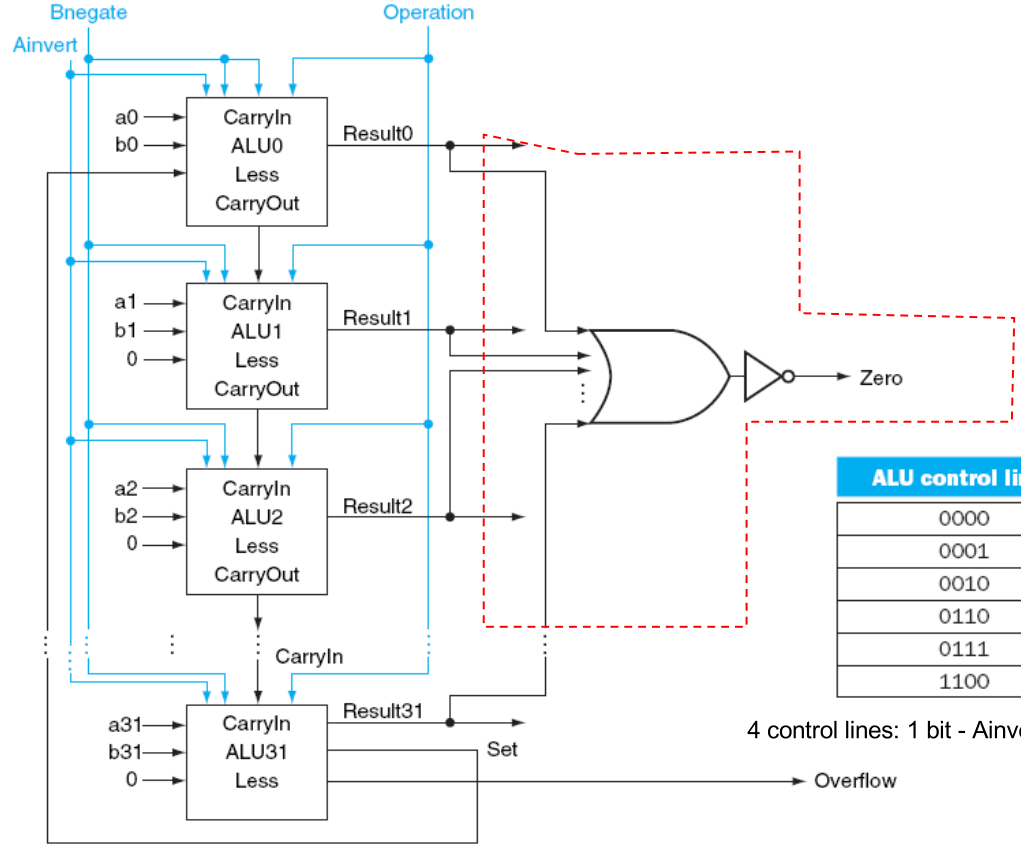
\includegraphics[scale=0.5]{Immagini/ALU-32Bit.png}
\end{center}

\begin{minipage}[t]{0.45\textwidth}
\subsection{Schema semplificato}
    \begin{center}
    \begin{tikzpicture}[font=\sffamily, thick, >=latex]
    
        % --- Corpo dell'ALU ---
        % Disegna il perimetro principale con l'intaglio a sinistra (forma a V)
        \draw[line width=1.5pt] (0, 0) -- (0, 5) -- (2, 3.8) -- (2, 1.2) -- cycle;
        
        % Intaglio centrale (V rovesciata sul dorso sinistro)
        \draw[fill=white, draw=none] (-0.1, 1.8) -- (0.6, 2.5) -- (-0.1, 3.2) -- cycle; % mask
        \draw[line width=1.5pt] (0, 3.2) -- (0.6, 2.5) -- (0, 1.8);
        
        \node at (1.1, 2.5) {ALU};
    
        % --- Ingressi a sinistra (a, b) ---
        \draw[->, line width=1.2pt] (-0.8, 4.0) node[left] {a} -- (0, 4.0);
        \draw[->, line width=1.2pt] (-0.8, 1.0) node[left] {b} -- (0, 1.0);
    
        % --- Ingresso dall'alto (ALU operation) in azzurro ---
        \node[text=cyan] at (1.0, 5.5) {ALU operation};
        \draw[->, cyan, line width=1.2pt] (1.0, 5.2) -- (1.0, 4.4);
    
        % --- Uscite a destra ---
        \draw[->, line width=1.2pt] (2.0, 3.2) -- (2.7, 3.2) node[right] {Zero};
        \draw[->, line width=1.2pt] (2.0, 2.5) -- (2.7, 2.5) node[right] {Result};
        \draw[->, line width=1.2pt] (2.0, 1.8) -- (2.7, 1.8) node[right] {Overflow};
    
        % --- Uscita in basso (CarryOut) ---
        \draw[->, line width=1.2pt] (1.0, 0.6) -- (1.0, -0.3) node[below] {CarryOut};
    
    \end{tikzpicture}
    \end{center}
\end{minipage}
\hfil
\begin{minipage}[t]{0.45\textwidth}
\subsection{Tabella di controllo}
    \begin{center}
    \begin{tabular}{|c|c|}
        \hline \textbf{Codice} & \textbf{Funzione} \\ \hline
        \texttt{0000} & AND \\ \hline
        \texttt{0001} & OR \\ \hline
        \texttt{0010} & ADD \\ \hline
        \texttt{0110} & SUB \\ \hline
        \texttt{0111} & SLT \\ \hline
        \texttt{1100} & NOR \\ \hline
    \end{tabular}
\end{center}
\end{minipage}

\subsection{Operazione BEQ - Branch on equal}

\subsubsection{Cosa fa?}

\vspace{0.5cm}

\begin{center}
    {
        \large
        \texttt{beq registro1, registro2, L1}
    }
\end{center}

\vspace{0.5cm}

L'istruzione ti fa saltare all'etichetta L1 se il valore contenuto in registro1 è uguale al valore contenuto in registro 2

\subsubsection{Come funziona?}
Per verificare l'uguaglianza di a e b si effettua una sottrazione

Se $a=b$ allora dobbiamo mettere a 1 la linea di output usata per l'uguagliaanza, oppure si fa l'OR di tutte le uscite e poi si nega il risultato
    \chapter{Reti sequenziali}

\section{Cosa è un circuito (o rete) sequenziale?}
Un circuito (o rete) sequenziale è un circuito in cui lo stato delle uscite non dipende solo dalla funzione logica applicata ai suoi ingressi, ma anche sulla base di valori pregressi collocati in memoria

\section{Componenti}
I circuiti sequenziali sono formati da:
\begin{itemize}
    \item Elementi di memoria (di vario tipo): Memorizzano l'informazione
    \item Reti combinatorie: Elaborano l'informazione
\end{itemize}

\section{Stato}
Un circuito sequenziale ha, in ogni dato istante, uno stato determinato dai bit memorizzati

\begin{center}
\begin{tikzpicture}[
    font=\sffamily,
    >=stealth,
    box/.style={draw, minimum width=3.5cm, minimum height=1.8cm, align=center},
    node distance=2.5cm
]

    % Definizione dei due blocchi principali
    \node[box] (mem) {Elementi \\ di memoria};
    \node[box, right=2cm of mem, yshift=1cm] (comb) {Circuito \\ combinatorio};

    % Ingressi
    % Creiamo una coordinata fittizia a sinistra per far partire la freccia degli Ingressi
    \coordinate (in_start) at ([xshift=-4.5cm]comb.165);
    \draw[->] (in_start) node[left] {Ingressi} -- (comb.165);

    % Uscite
    \draw[->] (comb.15) -- ++(1.5,0) node[right] {Uscite};

    % Stato Corrente (da mem a comb)
    \draw[->] (mem.east) -- (comb.195) node[midway, align=left, above] {Stato \\ corrente};

    % Stato Successivo (feedback da comb a mem)
    % Usiamo percorsi ortogonali (|- e -|) per fare il loop rettangolare verso il basso
    \draw[->] (comb.345) -- ++(1,0) |- ([yshift=-1cm]mem.south) -| ([xshift=-1cm]mem.west) -- (mem.west) 
        node[pos=0.15, above] {Stato successivo};

\end{tikzpicture}
\end{center}

\section{Famiglie di circuiti sequenziali}
Esistono 2 famiglie di circuiti digitali sequenziali:
\begin{itemize}
    \item \textbf{Asincroni}: Non fanno uso del clock
    \item \textbf{Sincroni}: Necessitano dell'utilizzo del clock
\end{itemize}

\newpage
\section{Clock}
\subsection{Cosa è?}
È un segnale (onda quadra) con periodo predeterminato e costante

\subsection{Diagramma}
\begin{center}
    \begin{tikzpicture}[font=\sffamily, >=latex, thick]

        % ==========================================
        % 1. Segnale di Clock (Onda quadra)
        % ==========================================
        \draw[line width=1.5pt] 
            (0,0) -- (1,0) -- (1,1.5) -- (3,1.5) -- (3,0) -- 
            (3.75,0) -- (3.75,1.5) -- (5.75,1.5) -- (5.75,0) -- 
            (6.5,0) -- (6.5,1.5) -- (8.5,1.5) -- (8.5,0);

        % ==========================================
        % 2. Indicatore del Periodo (Clock period)
        % ==========================================
        \draw[<->, line width=0.8pt] (1, -0.4) -- (3.75, -0.4);
        \node[below] at (2.375, -0.5) {Clock period};

        % ==========================================
        % 3. Indicatore Fronte di Salita (Rising edge)
        % ==========================================
        \draw[<-, line width=0.8pt] (3.75, 0.75) -- (4.6, -0.6);
        \node[right] at (4.5, -0.7) {Rising edge};

        % ==========================================
        % 4. Indicatore Fronte di Discesa (Falling edge)
        % ==========================================
        \draw[<-, line width=0.8pt] (5.75, 0.75) -- (6.5, 2.0);
        \node[right] at (6.4, 2.1) {Falling edge};

    \end{tikzpicture}
\end{center}

\subsection{Formula: Frequenza di clock}
\begin{center}
    \begin{tcolorbox}[title=Frequenza di clock,width=0.65\textwidth]
        {
            \Large
            $$
            F = \frac{1}{T}
            $$

            \begin{itemize}
                \item $T$ = Periodo / ciclo di clock
                \item $F$ = Frequenza di clock
            \end{itemize}
        }
    \end{tcolorbox}
\end{center}

\newpage
\section{S-R Latch}
\subsection{Cosa è?}
È un circuito composto da 2 porte NOR concatenate

\begin{minipage}{0.50\textwidth}
    \subsection{Schema}
    \begin{center}
        \begin{tikzpicture}[font=\Large\sffamily, line width=1.6pt, line cap=round, line join=round]

            % ==========================================
            % 1. Porta NOR Superiore
            % ==========================================
            \begin{scope}[shift={(0, 1.3)}]
                \draw (-0.1, -0.7) 
                    arc[start angle=-30, end angle=30, radius=1.4] 
                    arc[start angle=90, end angle=15, x radius=1.4, y radius=0.72]
                    arc[start angle=-15, end angle=-90, x radius=1.4, y radius=0.72] 
                    -- cycle;
                \draw (1.42, 0) circle (0.15);
                \draw (1.57, 0) -- (3.0, 0) node[right] {Q};
            \end{scope}

            % ==========================================
            % 2. Porta NOR Inferiore
            % ==========================================
            \begin{scope}[shift={(0, -1.3)}]
                \draw (-0.1, -0.7) 
                    arc[start angle=-30, end angle=30, radius=1.4] 
                    arc[start angle=90, end angle=15, x radius=1.4, y radius=0.72]
                    arc[start angle=-15, end angle=-90, x radius=1.4, y radius=0.72] 
                    -- cycle;
                \draw (1.42, 0) circle (0.15);
                \draw (1.57, 0) -- (3.0, 0) node[right] {$\overline{\mathsf{Q}}$};
            \end{scope}

            % ==========================================
            % 3. Ingressi Esterni (R e S)
            % ==========================================
            \draw (-1.8, 1.65) node[left] {R} -- (0.05, 1.65);
            \draw (-1.8, -1.65) node[left] {S} -- (0.05, -1.65);

            % ==========================================
            % 4. Cablaggio incrociato (Cross-Coupled Feedback)
            % ==========================================
            \fill (2.2, 1.3) circle (0.1);
            \fill (2.2, -1.3) circle (0.1);

            \draw (2.2, 1.3) -- (-1.0, -0.95) -- (0.05, -0.95);
            \draw (2.2, -1.3) -- (-1.0, 0.95) -- (0.05, 0.95);

        \end{tikzpicture}
    \end{center}
\end{minipage}
\hfil
\begin{minipage}{0.15\textwidth}
    \begin{center}
        {
            \Large
            S = Set

            R = Reset
        }
    \end{center}
\end{minipage}

\subsection{Tabella}
\begin{minipage}[t]{0.35\textwidth}
    \begin{center}
        \begin{tabular}{|c|c|c|c|c|}
            \hline
            \multicolumn{2}{|c|}{Input} & Stato Interno & \multicolumn{2}{c|}{Output} \\
            \multicolumn{1}{|c}{S} & \multicolumn{1}{c|}{R} & Old Q & \multicolumn{1}{c}{Q} & \multicolumn{1}{c|}{$\overline{\mathsf{Q}}$} \\
            \hline
            0 & 0 & 0 & 0 & 1 \\
            \hline
            0 & 0 & 1 & 1 & 0 \\
            \hline
            0 & 1 & 1/0 & 0 & 1 \\
            \hline
            1 & 0 & 1/0 & 1 & 0 \\
            \hline
            1 & 1 & 1/0 & 0 & 0 \\
            \hline
        \end{tabular}
    \end{center}
\end{minipage}
\hfil
\begin{minipage}{0.6\textwidth}
    \begin{itemize}
        \item La combinazione (S,R) = (0,0) viene detta combinazione di riposo, perchè semplicemente mantiente il valore memorizzato in precedenza
        
        \vspace{0.3cm}

        \item La combinazione (S,R) = (1,1) viola la proprietà di complementarietà di $Q$ e $\overline{Q}$, può portare ad una configurazione instabile
    \end{itemize}
\end{minipage}

\subsection{Problematiche}
In un SR Latch il valore di Q all'accensione dell'elaboratore è indeterminato, a meno che non ci sia un meccanismo di inizializzazione

\begin{itemize}
    \item All'accensione, i valori interni dei nodi dipendono da condizioni casuali, come la carica residua nei transisto o nei condensatori
    \item Se non viene forzato un valore iniziale, il latch potrebbe assumere un qualsiasi stato in modo casuale.
    \begin{itemize}
        \item \textbf{Reset Hardware}: Un segnale di reset globale può forzare $Q=0$ e $\overline{Q}=1$ subito dopo l'accensione
        \item \textbf{SR con Priorità di Reset}: Se il circuito include un reset attivo all'avvio, $Q$ sarà forzato a un valore noto
    \end{itemize}
\end{itemize}

\newpage
\section{D Latch}
\subsection{Definizione}
È un Latch sincronizzato con il clock, la sincronizzazione con il clock garantisce che il latch cambi stato solo in certi momenti

\subsection{Schema}
\begin{minipage}{0.4\textwidth}
    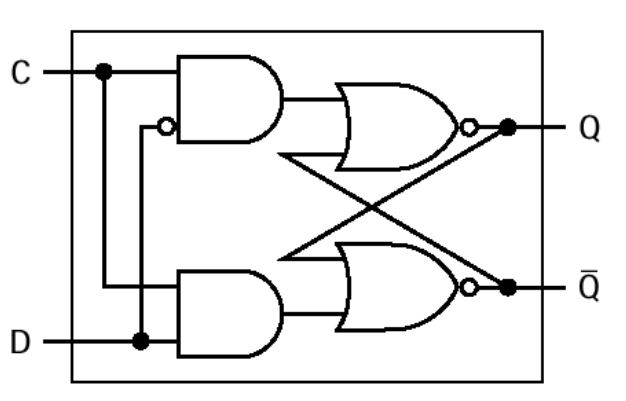
\includegraphics[scale=0.4]{Immagini/D-Latch.png}
\end{minipage}
\hfil
\begin{minipage}{0.45\textwidth}
    {
        \large

        \begin{itemize}
            \item $\mathbf{D=1}$ corrisponde al setting
            \begin{itemize}
                \item $S=1$ e $R=0$
            \end{itemize}
            \item $\mathbf{D=0}$ corrisponde al resetting
            \begin{itemize}
                \item $S=0$ e $R=1$
            \end{itemize}
        \end{itemize}
    }
\end{minipage}

\begin{center}
    \begin{itemize}
    \item Quando \textbf{il clock è deasserted} non viene memorizzato nessun valore:
    \begin{itemize}
        \item $S=0$ e $R=0$ (viene mantenuto il valore precedentemente memorizzato)
    \end{itemize}

    \item  Quando \textbf{il clock è asserted} viene memorizzato un valore (in funzione del valore di $D$)
    \end{itemize}
\end{center}

\subsection{Comportamento}
Il D-Latch è caratterizzato dal seguente comportamento:
\begin{enumerate}
    \item Durante l'intervallo alto del clock il valore del segnale di ingresso D viene memorizzato nel latch
    \item Il valore D si propaga quasi immediatamente all'uscita Q
    \item Anche le eventuali variazioni di D si propagano quasi immediatamente, con il risultato che Q può variare più volte durante l'intervallo alto del clock
    \item Solo quando il clock torno a zero Q si stabilizza
    \item Durante l'intervallo basso del clock il latch non memorizza
\end{enumerate}

\subsection{Segnale $D$}
Il segnale D ottenuto come output di un circuito combinatorio deve:
\begin{itemize}
    \item Essere già stabile quando $C$ diventa asserted
    \item Rimanere stabile per tutta la durata del livello alto di $C$ (Setup time)
    \item Rimanere stabile per un altro periodo di tempo per evitare malfunzionamenti (Hold time)
\end{itemize}

\begin{center}
    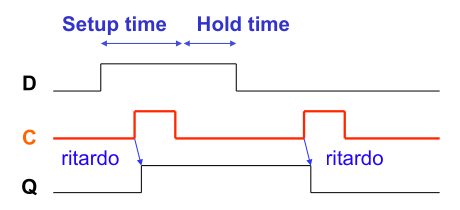
\includegraphics[scale=0.5]{Immagini/Segnale T.png}
\end{center}

\subsection{Lunghezza periodo di clock $T$}
Il periodo di clock $T$ deve essere scelto abbastanza lungo affinchè l'output del circuito combinatorio si stabilizzi

\begin{center}
    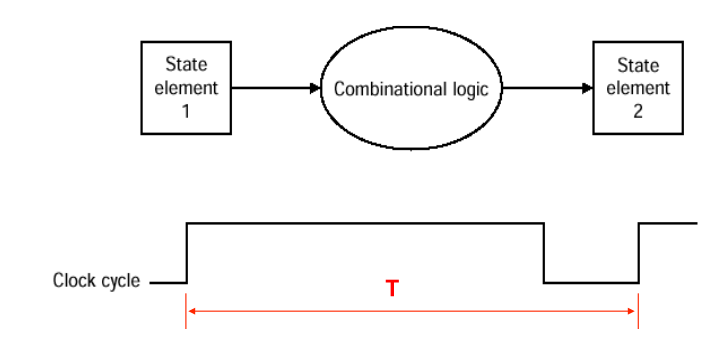
\includegraphics[scale=0.5]{Immagini/Lunghezza clock T.png}
\end{center}

\newpage
\section{D Flip-Flop}
\subsection{Metodologie di timing}
Fino ad ora abbiamo visto  una metodologia di timing detta \textbf{level-triggered} che avviene sul livello alto (o basso del clock)

Esiste una metodologia di timing chiamata \textbf{edge-triggered} che avviene sul fronte di salita (o di discesa) del clock
\begin{itemize}
    \item La memorizzazione avviene istantaneamente
    \item L'eventuale segnale di ritorno "sporco" non fa in tempo ad arrivare a causa dell'istantaneata della memorizzazione
\end{itemize}

\subsection{Definizione}
Il D Flip-Flop è usabile come input e output durante lo stesso ciclo di clock, viene realizzato ponendo in serie 2 D-Latch: il primo viene detto \textbf{master} e il secondo \textbf{slave}


\begin{minipage}[t]{0.45\textwidth}
    \subsection{Schema}
        \begin{center}
            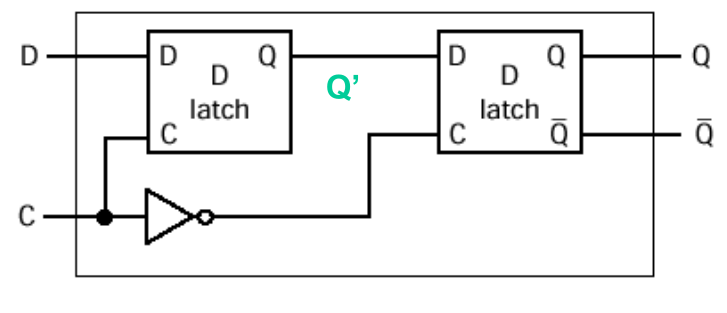
\includegraphics[scale=0.35]{Immagini/D FlipFlop Schema.png}
        \end{center}
    \subsection{Schema dei segnali}
        \begin{center}
            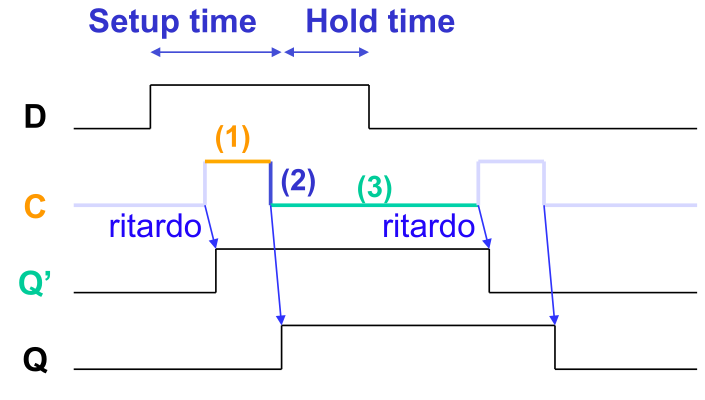
\includegraphics[scale=0.35]{Immagini/D FlipFlop Segnale.png}
        \end{center}
\end{minipage}
\hfil
\begin{minipage}[t]{0.45\textwidth}
    \subsection{Funzionamento}
        \begin{enumerate}
            \item Il primo latch è aperto e pronto per memorizzare D. \\
            Il valore memorizzato Q fluisce fuori, ma il secondo latch è chiuso 
            \begin{itemize}
                \item Nel circuito combinatorio a valle entra ancora il vecchio valore di Q
            \end{itemize}

            \item Il segnale del clock scende, e in questo istante il secondo latch viene aperto per memorizzare il valore di Q
            
            \item Il secondo latch è aperto, memorizza D, e fa fluire il nuovo valore Q nel circuito a valle.\\
            Il primo latch p invece chiuso, e non memorizza niente
        \end{enumerate}
\end{minipage}


    % 5) Datapath
    \chapter{Register File}

\section{Cosa è?}
Il Register File è una memoria veloce all'interno della CPU che contiene registri utilizzati per memorizzare dati temporanei durante l'esecuzione delle istruzioni

\section{Da cosa è composto?}
Ogni registro è costituito da:
\begin{itemize}
    \item \textbf{D Flip-Flop}: Per memorizzare ogni singolo bit
    \item \textbf{Multiplexer}: Per selezionare quale registro leggere o scrivere
    \item \textbf{Decoder}: Per indirizzare correttamente i registri
    \item \textbf{Circuiti di controllo}: Per gestire lettura/scrittura sincronizzate con il clock
\end{itemize}

\begin{minipage}[t]{0.45\textwidth}
    \subsection{Schema}
    \begin{center}
        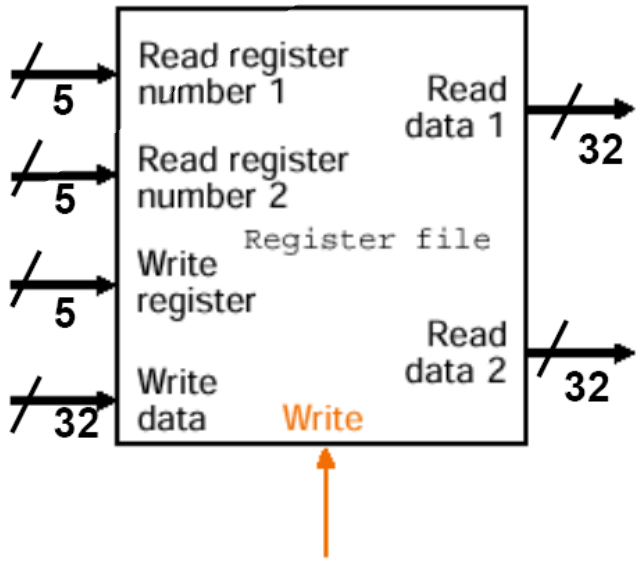
\includegraphics[scale=0.3]{Immagini/Register File.png}
    \end{center}
\end{minipage}
\hfil
\begin{minipage}[t]{0.45\textwidth}
    \subsection{Spiegazione porte}
    
    \subsubsection{Registri in lettura}
    \begin{itemize}
        \item \textbf{Read Reg1 (5 bit)}
        \begin{itemize}
            \item Numero del 1° registro da leggere
        \end{itemize}

        \item \textbf{Read Reg2 (5 bit)}
        \begin{itemize}
            \item Numero del 2° registro da leggere
        \end{itemize}

        \item \textbf{Read data 1 (32 bit)}
        \begin{itemize}
            \item Valore del 1° registro, letto sulla base di Read Reg1
        \end{itemize}

        \item \textbf{Read data 2 (32 bit)}
        \begin{itemize}
            \item Valore del 2° registro, letto sulla base di Read Reg2
        \end{itemize}
    \end{itemize}

    \subsubsection{Registri in scrittura}
    \begin{itemize}
        \item \textbf{Write Reg \# (5 bit)}
        \begin{itemize}
            \item Numero del registro da scrivere
        \end{itemize}

        \item \textbf{Write data (32 bit)}
        \begin{itemize}
            \item Valore da scrivere nel registro Write Reg \#
        \end{itemize}
    \end{itemize}

    \subsubsection{Segnali di controllo}
    \begin{itemize}
        \item \textbf{Write}
        \begin{itemize}
            \item Segnale di controllo messo in AND con il clock
            \item Solo se \texttt{Write=1}, il valore di Write data viene scritto in uno dei registri
        \end{itemize}
    \end{itemize}
\end{minipage}


\section{Lettura dal Register File}
\begin{minipage}[t]{0.45\textwidth}
    \subsection{Schema}
    \begin{center}
        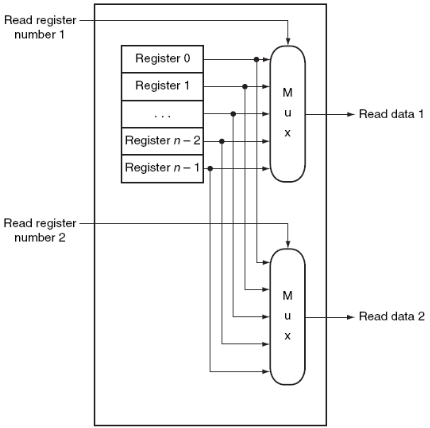
\includegraphics[scale=0.6]{Immagini/Lettura Register File.png}
    \end{center}
\end{minipage}
\hfil
\begin{minipage}[t]{0.45\textwidth}
    \subsection{Spiegazione}
    \begin{itemize}
        \item Utilizza 2 segnali che indicano i registri da leggere
        \item Utilizza 2 multiplexer: ognuno con 32 ingressi e un segnale di controllo
        \item Il register file fornisce sempre in output una coppia di registri
    \end{itemize}
\end{minipage}

\newpage
\section{Scrittura nel Register File}

\subsection{Schema}
\begin{center}
    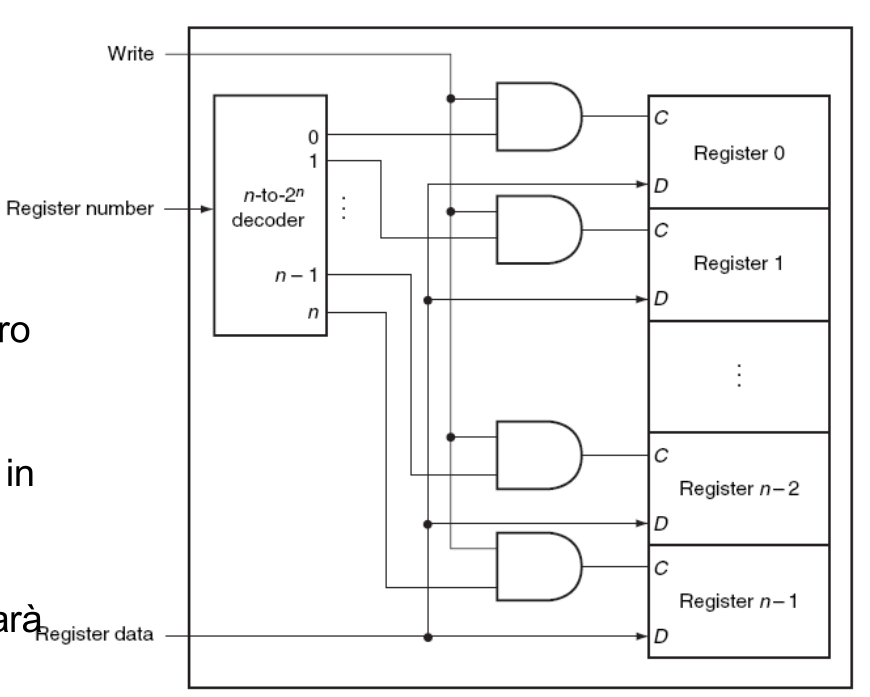
\includegraphics[scale=0.5]{Immagini/Scrittura Register File.png}
\end{center}

\subsection{Spiegazione}
\begin{itemize}
    \item Utilizza 3 segnali:
    \begin{itemize}
        \item Il registro da scrivere (Register Number)
        \item Il valore da scrivere (Register Data)
        \item Il segnale di controllo (Write)
    \end{itemize}

    \item Utilizza un decoder che decodfica il numero del registro da scrivere (Write Register)
    
    \item Il segnale Write (già un AND con il clock) è in AND con l'output del decoder
    
    \item Se Write non è affermato nessun valore sarà scritto nel registro
\end{itemize}
    \chapter{Datapath Multiciclo}

\section{Schema}
\begin{center}
    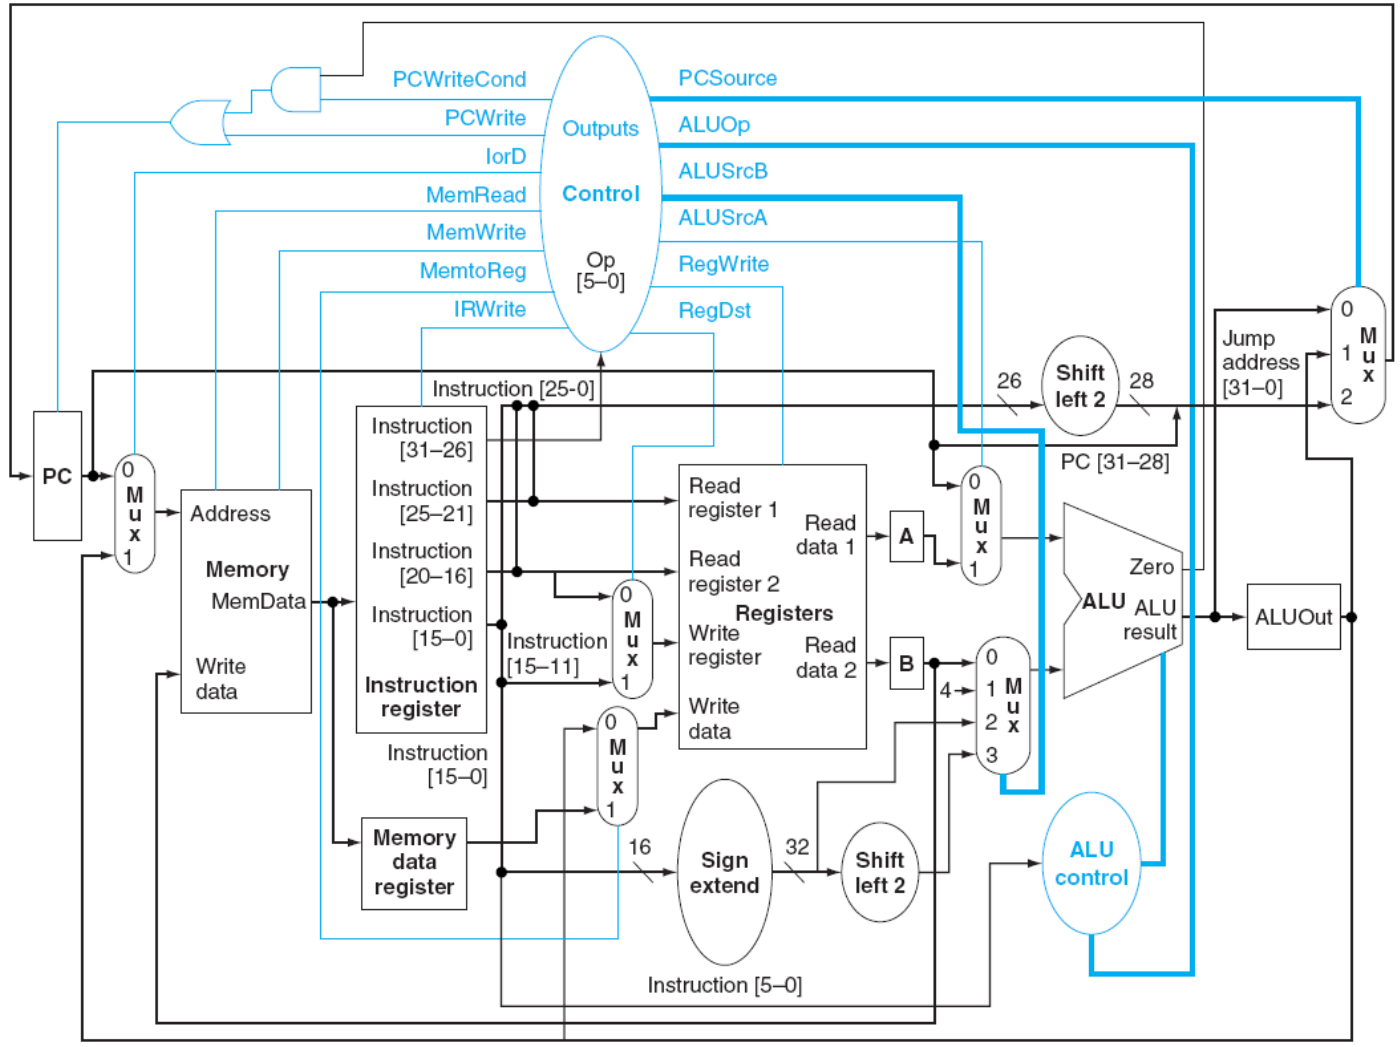
\includegraphics[scale=0.375]{Immagini/Datapath Multiciclo.png}
\end{center}

\newpage

\section{Componenti}
\subsection{Unità Funzionali}
\begin{itemize}
    \item \textbf{Memoria}: \\
        Un' unità unificata che contiene sia istruzioni che dati.\\
        Sulla base dell'indirizzo ricevuto in input, restituisce in output l'istruzione o il dato letto, oppure memorizza il dato (WriteData) nel caso di un'istruzione

    \item \textbf{Register File}: \\
        Un banco composto da 32 registri che contengono i dati utilizzati durante l'esecuzione delle istruzioni.\\
        Restituisce in output il contenuto dei due registri letti e, nel caso di istruzioni \texttt{load} o \texttt{R-Type}, scrive il dato ricevuto in input nel registro specificato

    \item \textbf{ALU}: \\
        Si occupa di eseguire le operazioni aritmetico-logiche richieste, come il calcolo del valore di branch o l'incremento del PC

    \item \textbf{Sign extend}: \\
        Unità per l'estensione del segno a 32 bit

    \item \textbf{Shift left 2}: \\
        Unità per scorrere i bit a sinistra di 2 posizioni
\end{itemize}

\subsection{Registri}
\begin{itemize}
    \item \textbf{PC - Program Counter}: \\
        Mantiene l'indirizzo dell'istruzione da eseguire

    \item \textbf{IR - Instruction Register}: \\
        Memorizza i bit dell'istruzione letta dalla memoria

    \item \textbf{Memory data register}: \\
        Memorizza il dato letto dalla memoria, utilizzato ad esempio per le istruzioni di tipo \texttt{load}

    \item \textbf{Registro A e Registro B}: \\
        Registri temporanei in cui vengono scritti i valori provenienti dal register file durante la fase di fetch (il valore del registro sorgente \texttt{\$ra} in A, il valore \texttt{\$rt} in B)

    \item \textbf{ALUOut}: \\
        Memorizza temporaneamente l'output generato dalla ALU
\end{itemize}

\subsection{Multiplexer}
Sono necessari per selezionare dinamicamente i percorsi dei dati nei diversi cicli di esecuzione

\begin{itemize}
    \item \textbf{MUX A}: \\
        Seleziona l'indirizzo di memoria a cui accedere tra il PC (per leggere un'istruzione) e l'output della ALU (per le istruzioni \texttt{load} o \texttt{store})

    \item \textbf{MUX B}: \\
        Seleziona il gruppo di bit dell'IR che indica il registro in cui scrivere (IR per le \texttt{load}, IR per le \texttt{R-Type})

    \item \textbf{MUX C}: \\
        Seleziona la sorgente del dato da scrivere nel register file (MemoryDataRegister per le \texttt{load}, ALUOut per le \texttt{R-Type})

    \item \textbf{MUX D}: \\
        Seleziona il primo operando dell'operazione aritmetico-logica della ALU tra il PC e il registro A

    \item \textbf{MUX E}: \\
        Seleziona il secondo operando della ALU tra il registro B, il valore costante 4, l'estensione in segno dell'IR[15:0], oppure l'estensione in sogno "2-shifted"

    \item \textbf{MUX F}: \\
        Seleziona il valore per l'aggionamento del PC tra l'output della ALU (PC + 4), il contenuto di ALUOut, o il jump target address
\end{itemize}

\section{Segnali di controllo}

\subsection{Segnali di Abilitazione (a 1 bit)}
Questi segnali controllano la scrittura o la lettura negli elementi di stato (memoria e registri). Un valore alto (1) attiva l'azione, un valore basso (0) la disabilita.

\begin{itemize}
    \item \textbf{MemRead}: Abilita la lettura dalla memoria principale.
    \begin{itemize}
        \item \textbf{1}: Legge l'istruzione o il dato dall'indirizzo specificato (utilizzato nello stato di \textit{fetch} per leggere l'istruzione o nell'istruzione \texttt{load}).
    \end{itemize}
    \item \textbf{MemWrite}: Abilita la scrittura nella memoria principale.
    \begin{itemize}
        \item \textbf{1}: Scrive il valore presente nell'ingresso "Write data" all'indirizzo specificato (utilizzato nell'istruzione \texttt{store}).
    \end{itemize}
    \item \textbf{IRWrite}: Abilita la scrittura nell'Instruction Register (IR).
    \begin{itemize}
        \item \textbf{1}: Memorizza l'istruzione appena letta dalla memoria (utilizzato solo nella fase di \textit{fetch}).
    \end{itemize}
    \item \textbf{RegWrite}: Abilita la scrittura nel Register File.
    \begin{itemize}
        \item \textbf{1}: Il dato presente in "Write data" viene scritto nel registro di destinazione selezionato (utilizzato alla fine delle istruzioni R-type, \texttt{load} o \texttt{swap}).
    \end{itemize}
    \item \textbf{PCWrite}: Abilita l'aggiornamento incondizionato del Program Counter (PC).
    \begin{itemize}
        \item \textbf{1}: Il PC memorizza un nuovo valore (utilizzato nel \textit{fetch} per salvare PC+4 o nei salti incondizionati come \texttt{jump}).
    \end{itemize}
    \item \textbf{PCWriteCond}: Abilita l'aggiornamento condizionato del Program Counter.
    \begin{itemize}
        \item \textbf{1}: Il PC viene aggiornato solo se la ALU restituisce il segnale \texttt{Zero = 1} (utilizzato per i salti condizionati come \texttt{beq}).
    \end{itemize}
\end{itemize}

\subsection{Segnali di Selezione Multiplexer a 2 vie (a 1 bit)}
Questi segnali fungono da selettori per i Multiplexer (MUX) che hanno due soli ingressi.

\begin{itemize}
    \item \textbf{IorD (MUX A)}: Seleziona la sorgente dell'indirizzo da inviare alla memoria.
    \begin{itemize}
        \item \textbf{0}: Seleziona il PC (utilizzato per leggere un'istruzione nella fase di \textit{fetch}).
        \item \textbf{1}: Seleziona l'output della ALU (utilizzato per l'esecuzione di istruzioni \texttt{load} o \texttt{store}).
    \end{itemize}
    \item \textbf{RegDst (MUX B)}: Seleziona quale parte dell'istruzione indica il registro in cui scrivere.
    \begin{itemize}
        \item \textbf{0}: Seleziona IR[20:16] (utilizzato per le istruzioni \texttt{load}).
        \item \textbf{1}: Seleziona IR[15:11] (utilizzato per le istruzioni R-type).
    \end{itemize}
    \item \textbf{ALUSrcA (MUX D)}: Seleziona il primo operando per la ALU.
    \begin{itemize}
        \item \textbf{0}: Seleziona il PC (utilizzato per l'incremento di +4 o per calcolare il valore di branch).
        \item \textbf{1}: Seleziona il registro A (utilizzato per istruzioni R-type, branch o \texttt{jump} con registro).
    \end{itemize}
    \item \textbf{MemtoReg (MUX C)}: Seleziona la sorgente del dato da scrivere nel register file.
    \begin{itemize}
        \item \textbf{0}: Seleziona ALUOut (utilizzato per le istruzioni R-type).
        \item \textbf{1}: Seleziona MemoryDataRegister (utilizzato per le istruzioni \texttt{load}).
        \item \textit{Nota}: In varianti dello schema (es. per l'istruzione \texttt{swap}), questo segnale può essere esteso a 2 bit per selezionare direttamente i registri A o B.
    \end{itemize}
\end{itemize}

\subsection{Segnali di Controllo a 2 bit (Multiplexer complessi e ALU)}
Questi segnali controllano Multiplexer a 3 o 4 vie, oppure l'unità di controllo della ALU.

\begin{itemize}
    \item \textbf{ALUSrcB (MUX E)}: Seleziona il secondo operando per la ALU.
    \begin{itemize}
        \item \textbf{00}: Seleziona il registro B (utilizzato per istruzioni R-type e branch).
        \item \textbf{01}: Seleziona la costante 4 (utilizzato per l'aggiornamento del PC nella fase di \textit{fetch}).
        \item \textbf{10}: Seleziona l'estensione del segno di IR[15:0] a 32 bit (utilizzato per istruzioni di accesso a memoria \texttt{lw}/\texttt{sw} o calcoli immediati).
        \item \textbf{11}: Seleziona l'estensione del segno di IR[15:0] shiftato a sinistra di 2 posizioni (utilizzato per pre-calcolare il valore di branch).
    \end{itemize}
    \item \textbf{PCSource (MUX F)}: Seleziona il valore con cui aggiornare il PC.
    \begin{itemize}
        \item \textbf{00}: Seleziona l'output diretto della ALU, ovvero PC+4.
        \item \textbf{01}: Seleziona il contenuto di ALUOut, ovvero l'indirizzo di branch calcolato (PC + 2 shifted sign-extended branch field).
        \item \textbf{10}: Seleziona il jump target address (indirizzo shiftato concatenato al PC).
    \end{itemize}
    \item \textbf{ALUOp}: Segnale inviato all'unità \texttt{ALU control} per decidere l'operazione aritmetico-logica da eseguire.
    \begin{itemize}
        \item \textbf{00}: Forza l'esecuzione di un'addizione (utilizzato nel \textit{fetch} per PC+4, nel \textit{decode}, e per il calcolo indirizzi memoria).
        \item \textbf{01}: Forza l'esecuzione di una sottrazione (utilizzato nello stato di esecuzione per verificare l'uguaglianza nel branch).
        \item \textbf{10}: Delega la decisione al campo \texttt{funct} (IR[5:0]) dell'istruzione (utilizzato per le istruzioni R-type).
    \end{itemize}
\end{itemize}

\subsection{Segnali per la Gestione delle Eccezioni (Co-processore 0)}
Quando il datapath viene esteso per gestire le eccezioni sincrone e asincrone, vengono aggiunti ulteriori segnali specifici controllati dalla FSM.

\begin{itemize}
    \item \textbf{EPCWrite}: Se a 1, abilita la scrittura dell'indirizzo dell'istruzione che ha causato l'eccezione nel registro \texttt{EPC}.
    \item \textbf{CauseWrite}: Se a 1, abilita la scrittura del tipo di eccezione nel registro \texttt{Cause}.
    \item \textbf{IntCause}: Identifica la causa specifica dell'eccezione (es. 0 per istruzione non valida, 1 per overflow aritmetico) per codificarla all'interno del registro \texttt{Cause}.
\end{itemize}

\section{Metodologia di clocking}
\begin{itemize}
    \item Ciclo di lunghezza fissa
    \item Ogni istruzione viene eseguita in più cicli di clock
    \item Istruzioni di tipo diverso vengono eseguito in un numero di cicli di clock diverso
    \item Le unità funzionali vengono usate più volte durante l'esecuzione della stessa istruzione in cicli di clock differenti
    \item Si usano registri aggiuntivi per memorizzare i risultati parziali nell'esecuzione delle istruzioni
\end{itemize}

\section{Passaggi per l'esecuzione di una istruzione}
\begin{enumerate}
    \item \textbf{Fetch}:
        \begin{enumerate}[label=\theenumi.\arabic*]
            \item Legge l'istruzione dalla memoria e la salva in un registro dedicato (IR - Instruction Register)
            \item L'indirizzo di memoria che indica l'istruzione da leggere si trova nel registro Program Counter (PC)
            \item Dopo la lettura dell'istruzione in PC viene incrementato di 4 (usando l'ALU) per indicare la prossima istruzione da leggere
        \end{enumerate}

    \item \textbf{Decode}:
        \begin{enumerate}[label=\theenumi.\arabic*]
            \item Decodificare i vari campi dell'istruzione per decidere quali sono i passi necessari per la sua esecuzione
        \end{enumerate}

    \item \textbf{Execute}:
        \begin{enumerate}[label=\theenumi.\arabic*]
            \item Esegue i passi necessari per eseguire l'istruzione
        \end{enumerate}
\end{enumerate}

Le operazioni di Fetch e Decode sono \textbf{uguali per tutti i tipi d'istruzione}, mentre l'operazione Execute dell'operazione di Execute cambia in base al tipo di istruzione da eseguire

\newpage

\section{FSM}
\begin{minipage}{0.45\textwidth}
    \subsection{Circuito sequenziale per il controllo}
    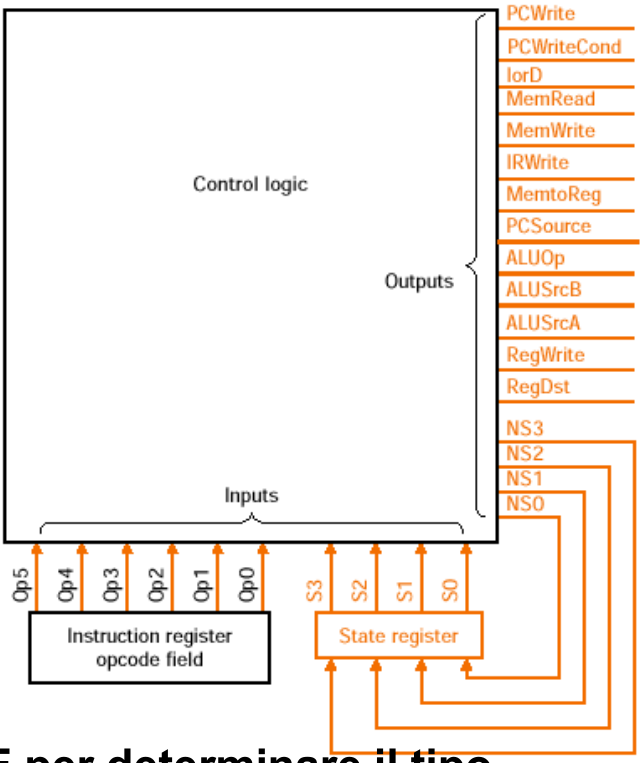
\includegraphics[scale=0.4]{Immagini/Schema FSM.png}
\end{minipage}
\hfil
\begin{minipage}{0.45\textwidth}
    \subsection{FSM}
    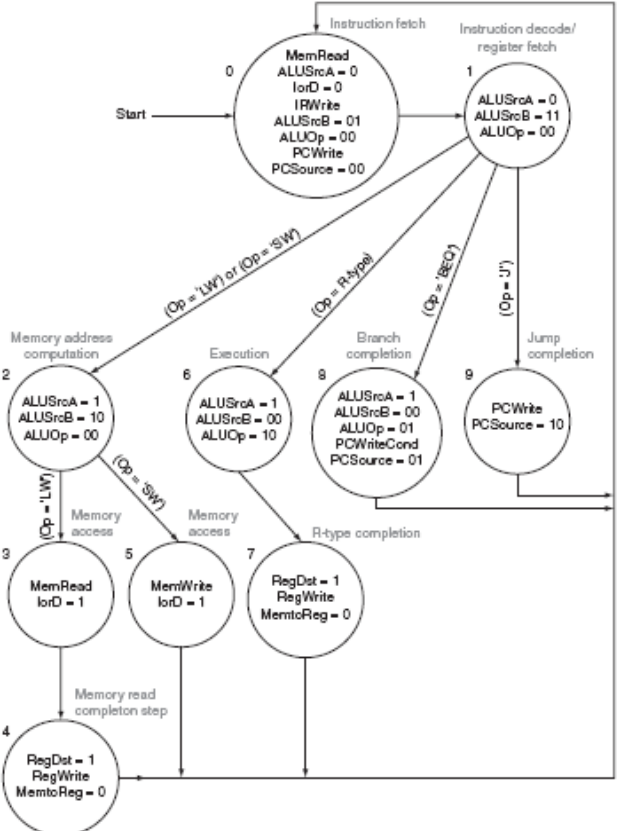
\includegraphics[scale=0.4]{Immagini/DFA SFM.png}
\end{minipage}

\subsection{Spiegazione}
\begin{itemize}
    \item Controllo a due livelli:
        \begin{itemize}
            \item Si usa \textbf{OPCODE} per determinare il tipo dell'istruzione
            \item Per le \uline{istruzioni R-Type} si usa anche il \textbf{funct}
        \end{itemize}
    
    \item State register memorizza lo stato corrente
    
    \item Blocco combinatorio (PLA) per il calcolo di NEXT\_STATE e OUTPUT
\end{itemize}

\newpage

\section{Fetch}
\subsection{Spiegazione}
Durante questo ciclo, il processore esegue contemporaneamente 2 compiti principali:
    \begin{itemize}
        \item Preleva l'istruzione dalla memoria
        \item Prepara il Program Counter (PC) per l'istruzione successiva
    \end{itemize}

L'intera operazione \uline{viene svolta in un singolo ciclo di clock}
\subsection{Componenti utilizzati}
\begin{itemize}
    \item Memoria
    \item Instruction Register
    \item Program Counter
    \item ALU
\end{itemize}


\subsection{Procedura}
\begin{enumerate}
    \item \textbf{Ciclo di clock 1}
        \begin{enumerate}[label=\theenumi.\arabic*]
            \item Usando l'indirizzo salvato all'interno del Program Counter prelevo l'istruzione da eseguire dalla memoria e la salvo all'interno dell'Instruction Register
            \item Utilizzando l'ALU aggiorno il PC a PC+4
        \end{enumerate}
\end{enumerate}

\subsection{Segnali}
\begin{itemize}
    \item \textbf{MemRead} per leggere dalla memoria
    \item \textbf{IRWrite} per scrivere nell'Instruction Register
    \item \textbf{IorD} per indicare da dove leggere dalla memoria
    \item \textbf{ALUSrcA, ALUSrcB, ALUop} per incrementare il PC
    \item \textbf{PCSource, PCWrite} per salvare il nuovo valore del PC al suo interno
\end{itemize}

\newpage

\section{Decode}
\subsection{Spiegazione}
Durante questo ciclo, il processore esegue contemporaneamente 2 compiti principali:
\begin{itemize}
    \item Il processore MIPS legge i vari campi dell'istruzione
    \item Il processore identifica il tipo di istruzione da eseguire usando l'opcode ed eventualmente anche il funct
\end{itemize}

L'intera operazione \uline{viene svolta in un singolo ciclo di clock}

\subsection{Componenti utilizzati}
\begin{itemize}
    \item Instruction Register
    \item Registro A
    \item Registro B
    \item ALUOut
    \item Sign Extend
\end{itemize}


\subsection{Procedura}
\begin{enumerate}
    \item[2.] \textbf{Ciclo di clock 2}
        \begin{enumerate}[label=\theenumi.\arabic*]
            \item [2.1] Il registro A usa i bit dal 25 al 21 dell'Instruction Register come eventuale dato per un istruzione futura
            \item [2.2] Il registro B usa i bit dal 20 al 16 dell'Instruction Register come eventuale dato per un istruzione futura
            \item [2.3] L'instruction register inserisci i bit dal 15 al 0 all'interno del sign extend e shift left 2, questo valore viene poi salvato all'interno di ALUOut per un eventuale calcolo di indirizzo di salto.
            \item [2.4] L'instruction register inserisce i bit dal 31 al 26 all'internodel FSM per decidere l'istruzione da effetuare utilizzando l'opcode
        \end{enumerate}
\end{enumerate}

\subsection{Segnali}
\begin{itemize}
    \item \textbf{ALUSrcA, ALUSrcB, ALUOp} per il calcolo di un eventuale indirizzo di branch
\end{itemize}

\newpage

\section{Execute per le istruzioni jump}
\subsection{Spiegazione}
Durante questa istruzione il processore esegue un solo compito:
\begin{itemize}
    \item Cambia l'indirizzo della prossima istruzione da eseguire con quella dell'indirizzo di salto calcolato durante la decode
\end{itemize}

L'intera istruzione \uline{viene completata in un singolo ciclo di clock}

\subsection{Componenti utilizzati}
\begin{itemize}
    \item Program Counter
    \item Instruction Register
\end{itemize}

\subsection{Procedura}
\begin{enumerate}
    \item[3.] \textbf{Ciclo di clock 3}
        \begin{enumerate}[label=\theenumi.\arabic*]
            \item [3.1] Il PC viene sovrascritto con l'indirizzo calcolato dall'ALU utilizzando i bit dal 31 al 28 del PC sommati ai bit dal 25 allo 0 dell'Instruction Register
        \end{enumerate}
\end{enumerate}

\subsection{Segnali}
\textbf{PCWrite, PCSource} per scrivere all'interno del PC

\newpage

\section{Execute beq}
\subsection{Spiegazione}
Durante questa istruzione il processore esegue 2 compiti:
\begin{itemize}
    \item Effettua il confronto tra i 2 valori 
    \item Eventualmente in base all'esito del confronto aggiorna il Program Counter
\end{itemize}

L'esecuzione di questa istruzione \uline{viene completata in un solo ciclo di clok}

\subsection{Componenti utilizzati}
\begin{itemize}
    \item Registro A
    \item Registro B
    \item ALUOut
\end{itemize}

\subsection{Procedura}
\begin{enumerate}
    \item[3.] \textbf{Ciclo di clock 3}
        \begin{enumerate}[label=\theenumi.\arabic*]
            \item [3.1] Il PC viene sovrascritto con l'indirizzo calcolato dall'ALU utilizzando i bit dal 31 al 
        \end{enumerate}
\end{enumerate}

\subsection{Segnali}
\begin{itemize}
    \item \textbf{ALUSrcA, ALUSrcB, ALUOp} per la comparazione tra A e B
    \item \textbf{PCWriteCond, PCSource} per scrivere all'interno del PC
\end{itemize}

\newpage

\section{Execute R-Type}
\subsection{Spiegazione}
Durante questa istruzione il processore esegue 2 compiti:

\begin{itemize}
    \item Effettuare l'operazione aritmetico logica definita dall'istruzione
    \item Salvare il risultato dell'operazione effettuata
\end{itemize}

L'esecuzione di questo tipo d'istruzioni \uline{dura 2 cicli di clock}

\subsection{Componenti utilizzati}
\begin{itemize}
    \item Registro A
    \item Registro B
    \item ALUOut
    \item Instruction Register
    \item Registro di destinazione dell'operazione
\end{itemize}

\subsection{Procedura}
\begin{enumerate}
    \item[3.] \textbf{Ciclo di clock 3}
        \begin{enumerate}[label=\theenumi.\arabic*]
            \item [3.1] Viene effettuata l'istruzione 
            \item [3.2] Il risultato dell'istruzione appena avvenuta viene salvato all'interno di ALUOut
        \end{enumerate}
    \item [4.] \textbf{Ciclo di clock 4}
        \begin{enumerate}
            \item [4.1] I contenuti di ALUOut vengono salvati nel registro di destinazione all'interno del Register file. L'indirizzo di questo registro di destinazione è specificato dai bit dal 15 all'11 dell'Instruction Register
        \end{enumerate}
\end{enumerate}

\subsection{Segnali}
\begin{itemize}
    \item \textbf{ALUScrA, ALUSrcB, ALUOp} per effettuare il calcolo aritmetico logico
    \item \textbf{RegWrite} per poter scrivere nel Register File
    \item \textbf{RegDest} per indicare il registro da scrivere
    \item \textbf{MemToReg} per scrivere il valore nel ALUOut
\end{itemize}

\newpage

\section{Execute Store Word}

\subsection{Spiegazione}
Durante questa istruzione il processore esegue 2 compiti:
\begin{itemize}
    \item Calcolare l'indirizzo dove salvare il dato
    \item Scrivere il dato in memoria
\end{itemize}

L'esecuzione di questa istruzione dura \uline{2 cicli di clock}

\subsection{Componenti utilizzati}
\begin{itemize}
    \item Registro A
    \item \textbf{Eventualmente} Registro B
    \item Sing extend
    \item Instruction Register
    \item ALUOut
    \item Memory data register \textbf{oppure} Memory
\end{itemize}

\subsection{Procedura}
\begin{enumerate}
    \item[3.] \textbf{Ciclo di clock 3}
        \begin{enumerate}[label=\theenumi.\arabic*]
            \item [3.1] Utilizzo il registro A e i bit dal 15 allo 0 dell'Instruction Register per calcolare l'indirizzo a in cui salvare il dato
            \item [3.2] Salvo l'indirizzo calcolato all'interno di ALUOut
        \end{enumerate}
    \item [4.] \textbf{Ciclo di clock 4}
        \begin{enumerate} [label=\theenumi.\arabic*]
            \item [4.1] In questo ciclo avviene l'effettiva scrittura del dato in memoria.\\ Per fare ciò, il multiplexer A seleziona l'output della ALU come indirizzo di memoria a cui accedere.\\ Il processore provvederà quindi a salvare in tale indirizzo il dato desiderato
        \end{enumerate}
\end{enumerate}

\subsection{Segnali di controllo}
\begin{itemize}
    \item \textbf{ALUSrcA, ALUSrcB, ALUOp} per il calcolo dell'indirizzo di memoria
    \item \textbf{IorD} per indicare l'indirizzo di memoria
    \item \textbf{MemWrite} per scrivere nella memoria
\end{itemize}

\newpage

\section{Execute Load Word}
\subsection{Spiegazione}
Durante questa istruzione il processore esegue 3 compiti:
\begin{itemize}
    \item Calcolare l'indirizzo dov'è contenuto il dato da leggere
    \item Legge il dato dalla memoria
    \item Riscrivere il dato appena letto all'interno del Register File
\end{itemize}

\subsection{Componenti utilizzati}
\begin{itemize}
    \item Registro A
    \item Registro B
    \item Sign extend
    \item Instruction Register
    \item ALUOut
    \item Memory Data Register
\end{itemize}

\subsection{Procedura}
\begin{enumerate}
    \item[3.] \textbf{Ciclo di clock 3}
        \begin{enumerate}[label=\theenumi.\arabic*]
            \item [3.1] Utilizzo il registro A e i bit dal 15 allo 0 dell'Instruction Register per calcolare l'indirizzo da cui leggere il dato
            \item [3.2] Salvo l'indirizzo calcolato all'interno di ALUOut
        \end{enumerate}
    \item [4.] \textbf{Ciclo di clock 4}
        \begin{enumerate} [label=\theenumi.\arabic*]
            \item [4.1] All'interno del Memory Data Register viene salvato il contenuto della cella di memoria con l'indirizzo salvato all'interno del registro ALUOut
        \end{enumerate}
    \item [5.] \textbf{Ciclo di clock 5}
        \begin{enumerate} [label=\theenumi.\arabic*]
            \item [5.1] In questo ultimo ciclo viene fatto il write back, riscrivendo all'interno del Instrucion Register nei bit dal 20 al 16 l'indirizzo in cui riscrivere i contenuti conservati all'interno del Memory Data Register
        \end{enumerate}
\end{enumerate}

\subsection{Segnali}
\begin{itemize}
    \item \textbf{ALUSrcA, ALUSrcB, ALUOp} per il calcolo dell'indirizzo di memoria
    \item \textbf{IorD} per indicare l'indirizzo di memoria
    \item \textbf{MemRead} per leggere dalla memoria
    \item \textbf{RegWrite} per poter scrivere nel Register File
    \item \textbf{RegDest} per indicare in registro da scrivere
    \item \textbf{MemToReg} per scrivere il valore dalla memoria
\end{itemize}
    \chapter{Datapath Singolo ciclo}

\section{Schema}
\begin{center}
    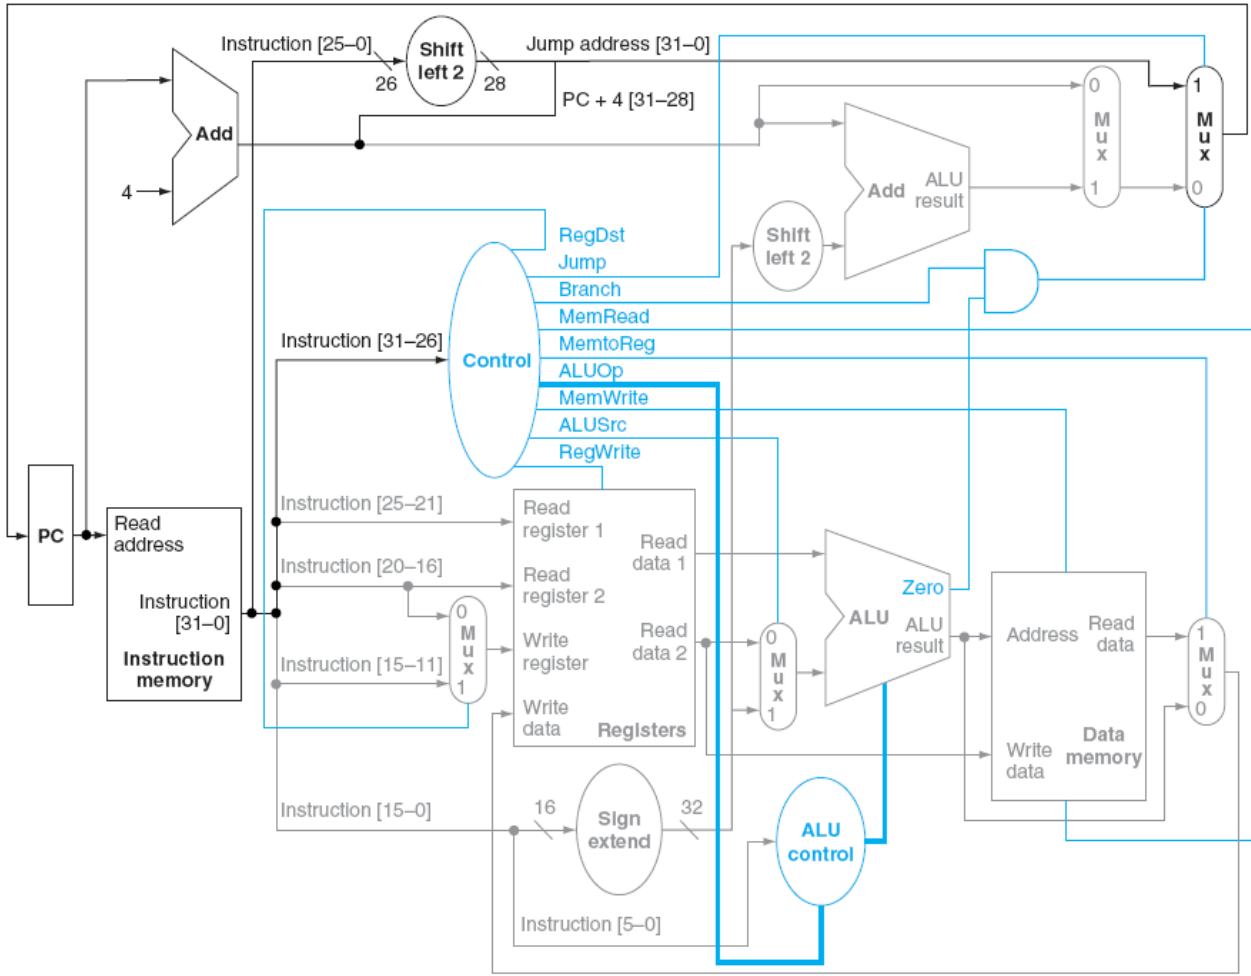
\includegraphics[scale=0.4]{Immagini/Schema Datapath Singolo Ciclo.png}
\end{center}

\section{Metodologia di clockin}
\begin{itemize}
    \item Ciclo di clock lungo (uguale al tempo necessario per eseguire l'istruzione più lunga)
    \item Istruzioni potenzialmente più veloci sono rallentate
    \item Unità funzionali replicate
\end{itemize}

    % 6) Eccezioni
    \chapter{Eccezioni}

\section{Definizione}
Un eccezione è un evento \textbf{sincrono}, generato all'interno del processore e provocato da problemi nell'esecuzione di un'istruzione

\subsection{Esempi di eccezioni}
\begin{itemize}
    \item Overflow
    \item Istruzione non valida
    \item Errori
    \item Pagine non presenti
    \item \dots
\end{itemize}

\section{Procedura generale per la gestione di un eccezione}

\subsection{Procedura generale}
\begin{enumerate}
    \item Interruzione dell'esecuzione del programma corrente
    \item Salvataggio parziale dello stato di esecuzione corrente per riprendere eventualmente l'esecuzione del programma corrente se possibile
    \item Salto a una routine del sistema operativo per gestire l'eccezione (tale routine è chiama di solito exception handler)
    \item Esecuzione della routine del SO
    \item Se possibile, ripristino dello stato di esecuzione del programma e continuazione dell'esecuzione del programma
\end{enumerate}

\subsection{Problematica: Identificazione dell'evento inatteso}
Per capire quale sia l'evento inatteso verificatosi si hanno 2 possibili soluzioni

\subsubsection{Indirizzo fisso}
Il controllo della CPU, prima di saltare all'handler del SO (a un indirizzo fisso), deve saltare in un registro interno un identificatore numerico del tipo di eccezione verificatosi.

L'handler accederà al registro interno per determinare la causa dell'eccezione

\subsubsection{Interruzioni vettorizzate}
Il controllo della CPU sceglie l'handler corretto, saltando all'indirizzo corretto.

A questo scopo, viene predisposto un vettore di indirizzi, uno per ogni tipo di eccezione, da indirizzare tramite il codice numerico dell'eccezione

\vspace{0.3cm}

\begin{center}
    \begin{tabular}{|c|c|}
        \hline \textbf{Tipo di eccezione} & \textbf{Exception vector address (in hex)} \\ \hline

        Undefined Instruction & $\texttt{C000\ 0000}_{hex}$ \\ \hline

        Arithmetic Overflow & $\texttt{C000\ 0020}_{hex}$ \\ \hline
        
    \end{tabular}
\end{center}

\section{Gestione delle eccezioni in MIPS}

\subsection{Registri Coprocessore 0}
Nel MIPS viene adottata la prima soluzione

\begin{itemize}
    \item Il registro \textbf{Cause} viene usato per memorizzare il motivo dell'eccezione
    
        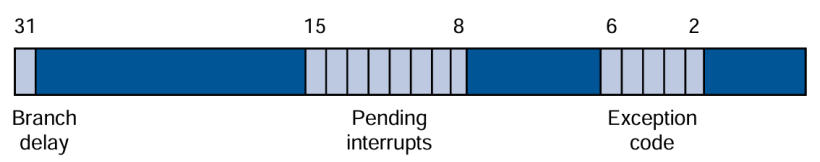
\includegraphics[scale=0.5]{Immagini/Registro cause.png}

    \item Il registro \textbf{EPC - Exception Program Counter} viene usato per memorizzare l'indirizzo dell'istruzione corrente che ha causato l'eccezione 
    \item Il registro \textbf{Status} viene usato per memorizzare la maschera delle interruzioni e bit di abilitazione
    
        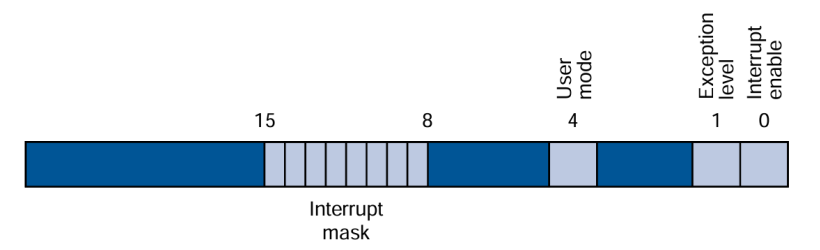
\includegraphics[scale=0.5]{Immagini/Registro Status.png}

    \item Il registro \textbf{BadVAddr} viene usato per memorizzare l'indirizzo di memoria il cui riferimento ha provocato l'eccezione
\end{itemize}

\subsection{Procedura}
    \subsubsection{Azioni a carico dell'hardware}
    \begin{enumerate}
        \item Individuare l'evento inatteso, la causa dell'eccezione e salvarla all'interno del registro Cause
        \item Interrompere l'esecuzione corrente
        \item Salvare l'indirizzo dell'istruzione corrente nel EPC ($EPC = PC-4$)
        \item Saltare all'indirizzo dell'exception handler
    \end{enumerate}

    \subsubsection{Azioni a carico dell'exception handler}
    \begin{enumerate}
        \item [4.] L'Exception Handler salva in memoria lo stato dei registri general purpose che intende utilizzare durante l'elaborazione, ad eccezione dei registri riservati $k0 e $k1. Non si salvano i registri del coprocessore, semmai se ne legge il contenuto.
        \item [5.] Gestisce l'eccezione, dopodiché ripristina dalla memoria i registri general purpose salvati in precedenza ed esegue l'istruzione eret per ritornare al programma originale, riprendendo l'esecuzione dall'indirizzo specificato da EPC
    \end{enumerate}


\subsection{Tabella delle eccezioni}
\begin{center}
    \begin{tabular}{|c|l|l|}
    \hline
    \textbf{Number} & \textbf{Name} & \textbf{Cause of exception} \\
    \hline
    0 & Int & interrupt (hardware) \\
    \hline
    4 & AdEL & address error exception (load or instruction fetch) \\
    \hline
    5 & AdES & address error exception (store) \\
    \hline
    6 & IBE & bus error on instruction fetch \\
    \hline
    7 & DBE & bus error on data load or store \\
    \hline
    8 & Sys & syscall exception \\
    \hline
    9 & Bp & breakpoint exception \\
    \hline
    10 & RI & reserved instruction exception \\
    \hline
    11 & CpU & coprocessor unimplemented \\
    \hline
    12 & Ov & arithmetic overflow exception \\
    \hline
    13 & Tr & trap \\
    \hline
    15 & FPE & floating point \\
    \hline
    \end{tabular}
\end{center}

    % 7) Interruzioni
    \chapter{Interrupt}

\section{Definizione}
Un Interrupt è un evento \textbf{asincrono} che giunge dall'esterno del processore, solitamente è un unità di I/O utilizzata per comunicare alla CPU il verificarsi di certi eventi



    \chapter{I/O gestito da programma}
    \chapter{I/O gestito da interrupt}
    \chapter{I/O gestito da DMA}


    % 8) Gerarchie di memoria

% --- ESERCITAZIONI SVOLTE
\part{Esercitazioni svolte} \setcounter{chapter}{0}


% --- Laboratori Svolti
\part{Laboratori svolti} \setcounter{chapter}{0}

% --- QUIZ MEGA SVOLTI
\part{Quiz Mega svolti} \setcounter{chapter}{0}

% --- Domande Aperte Mega Svolte
\part{Domande aperte Mega svolte} \setcounter{chapter}{0}


\end{document}